% Options for packages loaded elsewhere
\PassOptionsToPackage{unicode}{hyperref}
\PassOptionsToPackage{hyphens}{url}
\PassOptionsToPackage{dvipsnames,svgnames,x11names}{xcolor}
%
\documentclass[
  letterpaper,
  DIV=11,
  numbers=noendperiod]{scrartcl}

\usepackage{amsmath,amssymb}
\usepackage{lmodern}
\usepackage{iftex}
\ifPDFTeX
  \usepackage[T1]{fontenc}
  \usepackage[utf8]{inputenc}
  \usepackage{textcomp} % provide euro and other symbols
\else % if luatex or xetex
  \usepackage{unicode-math}
  \defaultfontfeatures{Scale=MatchLowercase}
  \defaultfontfeatures[\rmfamily]{Ligatures=TeX,Scale=1}
\fi
% Use upquote if available, for straight quotes in verbatim environments
\IfFileExists{upquote.sty}{\usepackage{upquote}}{}
\IfFileExists{microtype.sty}{% use microtype if available
  \usepackage[]{microtype}
  \UseMicrotypeSet[protrusion]{basicmath} % disable protrusion for tt fonts
}{}
\makeatletter
\@ifundefined{KOMAClassName}{% if non-KOMA class
  \IfFileExists{parskip.sty}{%
    \usepackage{parskip}
  }{% else
    \setlength{\parindent}{0pt}
    \setlength{\parskip}{6pt plus 2pt minus 1pt}}
}{% if KOMA class
  \KOMAoptions{parskip=half}}
\makeatother
\usepackage{xcolor}
\setlength{\emergencystretch}{3em} % prevent overfull lines
\setcounter{secnumdepth}{-\maxdimen} % remove section numbering
% Make \paragraph and \subparagraph free-standing
\ifx\paragraph\undefined\else
  \let\oldparagraph\paragraph
  \renewcommand{\paragraph}[1]{\oldparagraph{#1}\mbox{}}
\fi
\ifx\subparagraph\undefined\else
  \let\oldsubparagraph\subparagraph
  \renewcommand{\subparagraph}[1]{\oldsubparagraph{#1}\mbox{}}
\fi


\providecommand{\tightlist}{%
  \setlength{\itemsep}{0pt}\setlength{\parskip}{0pt}}\usepackage{longtable,booktabs,array}
\usepackage{calc} % for calculating minipage widths
% Correct order of tables after \paragraph or \subparagraph
\usepackage{etoolbox}
\makeatletter
\patchcmd\longtable{\par}{\if@noskipsec\mbox{}\fi\par}{}{}
\makeatother
% Allow footnotes in longtable head/foot
\IfFileExists{footnotehyper.sty}{\usepackage{footnotehyper}}{\usepackage{footnote}}
\makesavenoteenv{longtable}
\usepackage{graphicx}
\makeatletter
\def\maxwidth{\ifdim\Gin@nat@width>\linewidth\linewidth\else\Gin@nat@width\fi}
\def\maxheight{\ifdim\Gin@nat@height>\textheight\textheight\else\Gin@nat@height\fi}
\makeatother
% Scale images if necessary, so that they will not overflow the page
% margins by default, and it is still possible to overwrite the defaults
% using explicit options in \includegraphics[width, height, ...]{}
\setkeys{Gin}{width=\maxwidth,height=\maxheight,keepaspectratio}
% Set default figure placement to htbp
\makeatletter
\def\fps@figure{htbp}
\makeatother

\KOMAoption{captions}{tableheading}
\makeatletter
\makeatother
\makeatletter
\makeatother
\makeatletter
\@ifpackageloaded{caption}{}{\usepackage{caption}}
\AtBeginDocument{%
\ifdefined\contentsname
  \renewcommand*\contentsname{Table of contents}
\else
  \newcommand\contentsname{Table of contents}
\fi
\ifdefined\listfigurename
  \renewcommand*\listfigurename{List of Figures}
\else
  \newcommand\listfigurename{List of Figures}
\fi
\ifdefined\listtablename
  \renewcommand*\listtablename{List of Tables}
\else
  \newcommand\listtablename{List of Tables}
\fi
\ifdefined\figurename
  \renewcommand*\figurename{Figure}
\else
  \newcommand\figurename{Figure}
\fi
\ifdefined\tablename
  \renewcommand*\tablename{Table}
\else
  \newcommand\tablename{Table}
\fi
}
\@ifpackageloaded{float}{}{\usepackage{float}}
\floatstyle{ruled}
\@ifundefined{c@chapter}{\newfloat{codelisting}{h}{lop}}{\newfloat{codelisting}{h}{lop}[chapter]}
\floatname{codelisting}{Listing}
\newcommand*\listoflistings{\listof{codelisting}{List of Listings}}
\makeatother
\makeatletter
\@ifpackageloaded{caption}{}{\usepackage{caption}}
\@ifpackageloaded{subcaption}{}{\usepackage{subcaption}}
\makeatother
\makeatletter
\@ifpackageloaded{tcolorbox}{}{\usepackage[many]{tcolorbox}}
\makeatother
\makeatletter
\@ifundefined{shadecolor}{\definecolor{shadecolor}{rgb}{.97, .97, .97}}
\makeatother
\makeatletter
\makeatother
\ifLuaTeX
  \usepackage{selnolig}  % disable illegal ligatures
\fi
\IfFileExists{bookmark.sty}{\usepackage{bookmark}}{\usepackage{hyperref}}
\IfFileExists{xurl.sty}{\usepackage{xurl}}{} % add URL line breaks if available
\urlstyle{same} % disable monospaced font for URLs
\hypersetup{
  pdftitle={Effects of Misinformation on Online Discussions},
  pdfauthor={Jula Luehring},
  colorlinks=true,
  linkcolor={blue},
  filecolor={Maroon},
  citecolor={Blue},
  urlcolor={Blue},
  pdfcreator={LaTeX via pandoc}}

\title{Effects of Misinformation on Online Discussions}
\usepackage{etoolbox}
\makeatletter
\providecommand{\subtitle}[1]{% add subtitle to \maketitle
  \apptocmd{\@title}{\par {\large #1 \par}}{}{}
}
\makeatother
\subtitle{CSH Friday talk}
\author{Jula Luehring}
\date{14 June 2024}

\begin{document}
\maketitle
\ifdefined\Shaded\renewenvironment{Shaded}{\begin{tcolorbox}[breakable, sharp corners, enhanced, boxrule=0pt, interior hidden, borderline west={3pt}{0pt}{shadecolor}, frame hidden]}{\end{tcolorbox}}\fi

\hypertarget{misinformation-and-emotions}{%
\subsection{Misinformation and
emotions}\label{misinformation-and-emotions}}

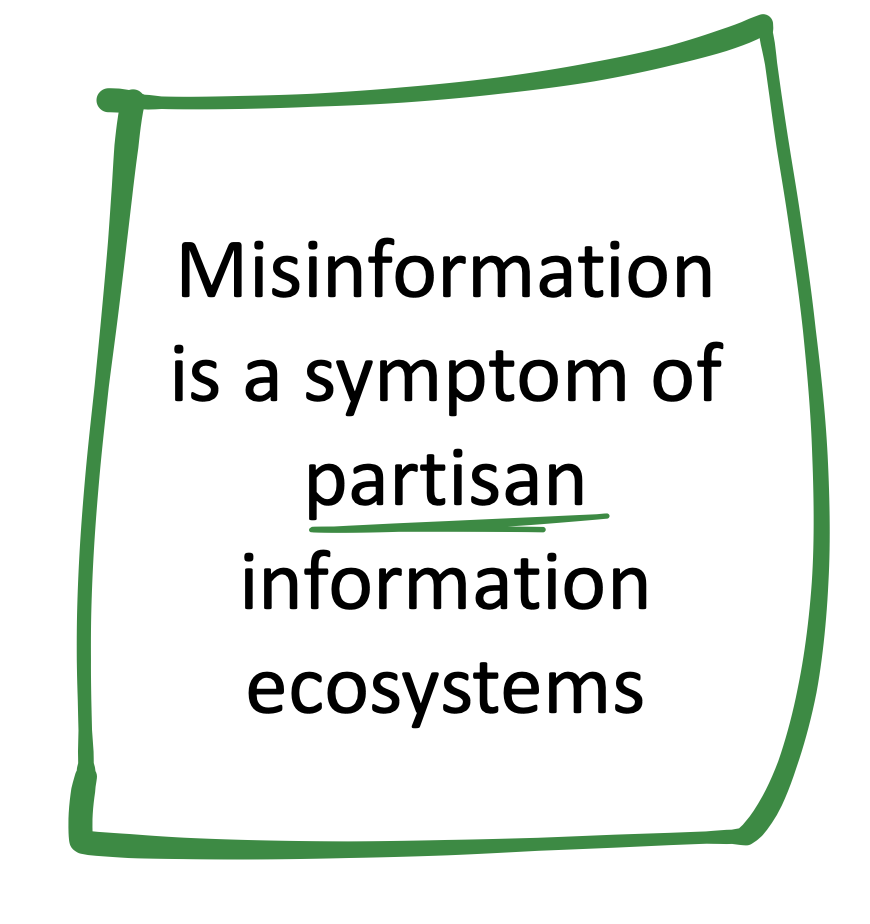
\includegraphics[width=10.41667in,height=\textheight]{images/misinfo-theory.png}

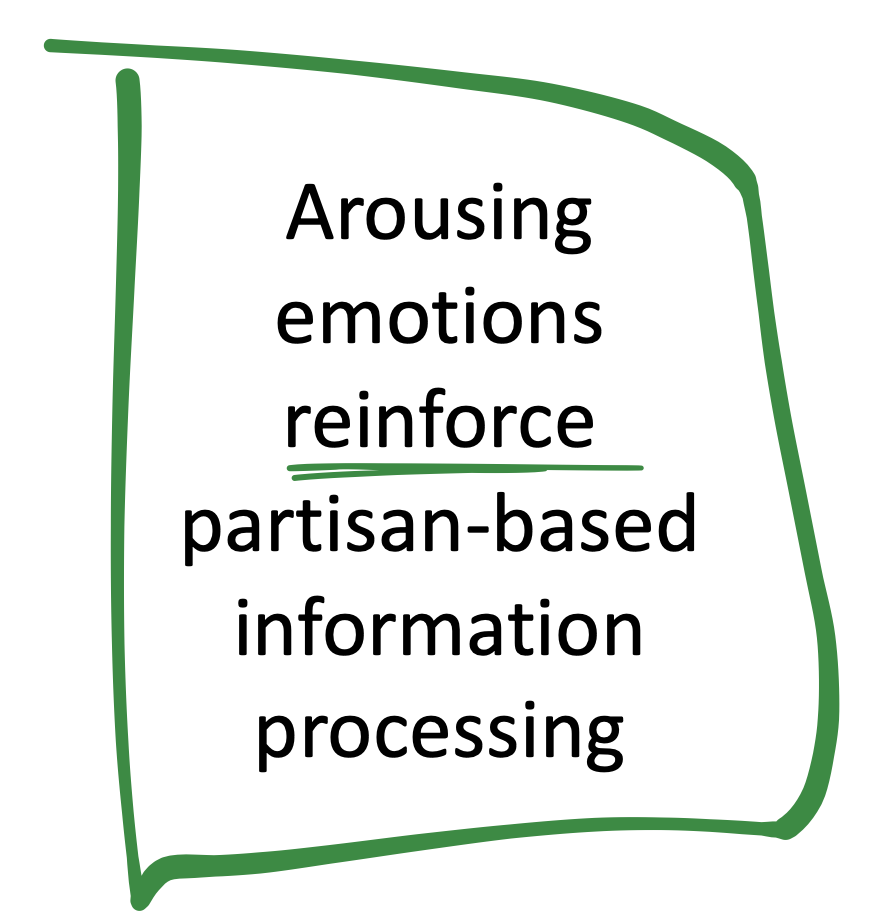
\includegraphics[width=10.41667in,height=\textheight]{images/emotion-theory.png}

Altay et al., \href{https://doi.org/10.1177/20563051221150412}{2023};
Ecker et al.,
\href{https://www.nature.com/articles/s44159-021-00006-y}{2023}; Martel
et
al.~\href{https://www.ncbi.nlm.nih.gov/pmc/articles/PMC7539247/}{2020};
Wardle \& Derakhshan,
\href{http://tverezo.info/wp-content/uploads/2017/11/PREMS-162317-GBR-2018-Report-desinformation-A4-BAT.pdf}{2017}

\begin{itemize}
\item
  So when we talk about misinformation, we usually refer to inaccurate
  information, regardless of the intention.
\item
  People have a lot of reasons to believe in misinformation, but there
  is more and more evidence showing that one of the strongest predictors
  is partisanship
\item
  Therefore, misinformation is now understood as a symptom of a
  clustered information ecosystem where few people are exposed to
  misinformation, while most people have partisan information diets,
  including decontextualized but not completely inaccurate information
\item
  In partisan-based information processing, emotions play a very
  important role
\item
  While arousing, mobilizing emotions signal us to better select,
  process and memorize vital information
\item
  Which, in theory, is good, they can also hinder systematic processing
\item
  In the case of misinformation, arousing emotions may therefore
  reinforce partisan-based processing
\end{itemize}

\hypertarget{do-arousing-emotions-make-people-believe-in-misinformation}{%
\section{Do (arousing) emotions make people believe in
misinformation?}\label{do-arousing-emotions-make-people-believe-in-misinformation}}

\hypertarget{emotional-state}{%
\subsection[Emotional state ]{\texorpdfstring{Emotional state
\protect
\includegraphics[width=3.125in,height=\textheight]{images/simple-relationship.png}}{Emotional state }}\label{emotional-state}}

\begin{itemize}
\item
  Replication study
\item
  False/accurate COVID-19 news headlines
\item
  Austria 2021
\item
  \emph{N} = 422
\end{itemize}

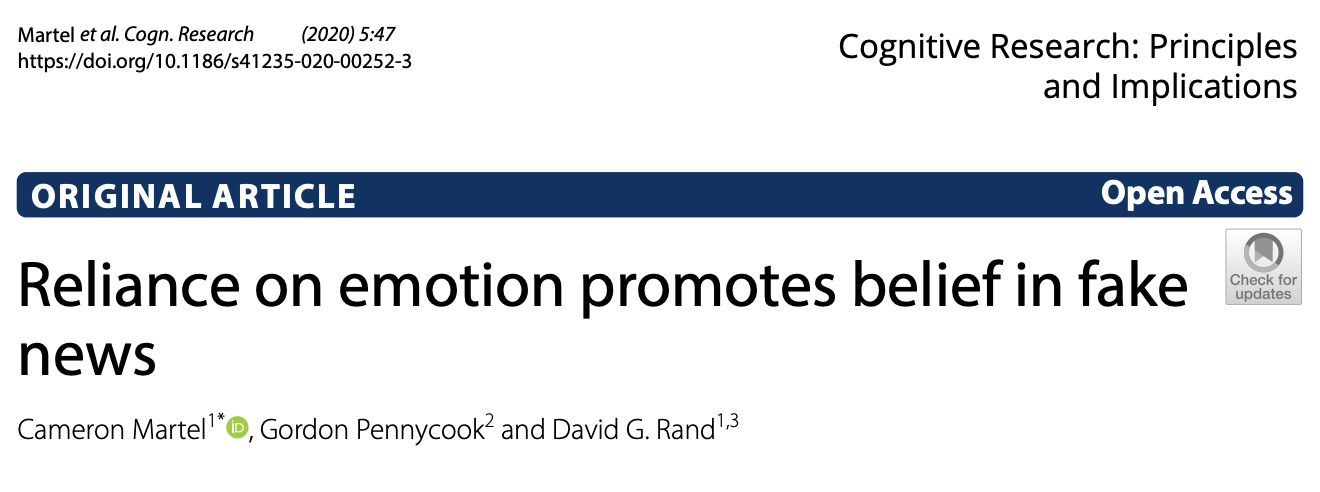
\includegraphics[width=10.41667in,height=\textheight]{images/Martel.png}

\(\rightarrow\) No effects of emotional state on misinformation
acceptance

Luehring*, Shetty*, et al., \href{https://psyarxiv.com/udqms/}{2023};
Martel et al.,
\href{https://link.springer.com/article/10.1186/s41235-020-00252-3}{2020}

\hypertarget{emotional-response}{%
\subsection{Emotional response}\label{emotional-response}}

\(\rightarrow\) More anger and less joy in response to false news

🗯 \emph{``Bullshit'', ``Fake''}

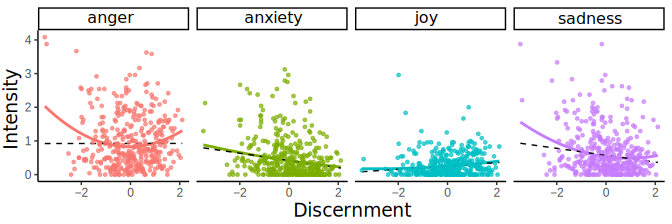
\includegraphics[width=8.33333in,height=\textheight]{images/curvi-linear.svg}

\(\rightarrow\) Function of emotion depends on existing beliefs

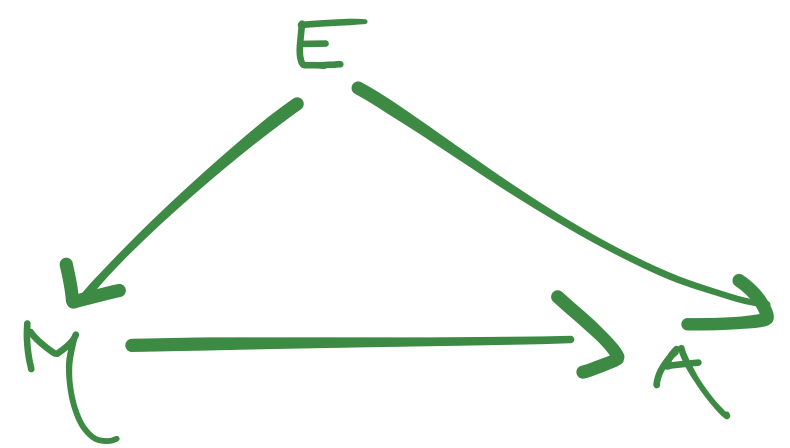
\includegraphics[width=3.125in,height=\textheight]{images/mediating-relationship.png}

Luehring*, Shetty*, et al., \href{https://psyarxiv.com/udqms/}{2023};
Van Damme \& Smets,
\href{https://psycnet.apa.org/record/2013-39652-001}{2014}

But we also looked at the emotional response as a more immediate measure
of emotions and we found more anger and less joy in response to the
false items

However, we also included some open-ended items and we found that people
reacted with disbelief, they said things like bullshit or nonse

So here in this plot you can see a non-linear relationship between
discernment and anger, and we can see that people who were really good
at discerning true from false and the ones who were really bad at it got
angry

Therefore, the function of emotions depends on prior beliefs and it
mediates the effect of misinformation

\hypertarget{problem-1}{%
\subsection{Problem \#1}\label{problem-1}}

Different effects of emotions are overlooked by

\begin{itemize}
\item
  mixing up different timings of emotions,
\item
  ignoring the function of emotions,
\item
  measuring positive and negative sentiment only.
\end{itemize}

\hypertarget{misinformation-on-social-media}{%
\section{Misinformation on social
media}\label{misinformation-on-social-media}}

\hypertarget{collective-dynamics-online}{%
\subsection{Collective dynamics
online}\label{collective-dynamics-online}}

\begin{itemize}
\item
  Moralizing and arousing content gets high engagement
\item
  Misinformation: conflict and negative

  \begin{itemize}
  \tightlist
  \item
    \textbf{But:} only 0.3-6\% in 5 studies from 2016-2021
  \item
    Elite and ordinary partisan superspreaders
  \end{itemize}
\end{itemize}

\(\rightarrow\) Misinformation is embedded in partisan intergroup
dynamics

\(\rightarrow\) Secondary effects?

\begin{figure}

{\centering 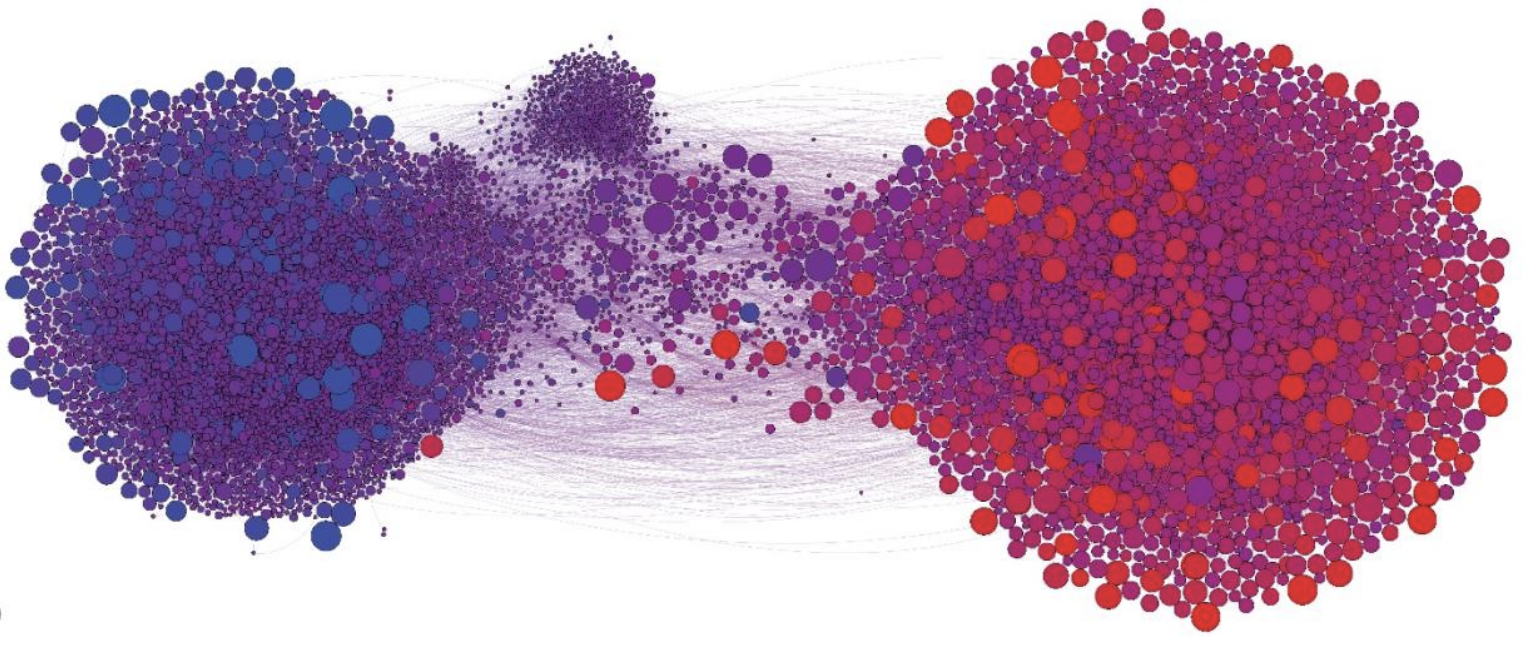
\includegraphics[width=6.25in,height=\textheight]{images/Nikolov.png}

}

\caption{Nikolov et al.,
\href{https://misinforeview.hks.harvard.edu/wp-content/uploads/2021/02/nikolov_partisanship_vulnerability_misinformation_20210215.pdf}{2021}}

\end{figure}

Allen et al.,
\href{https://www.science.org/doi/full/10.1126/science.adk3451}{2024};
Bail,
\href{https://press.princeton.edu/books/hardcover/9780691203423/breaking-the-social-media-prism}{2021};
Baribi-Bartov et al.,
\href{https://www.science.org/doi/10.1126/science.adl4435}{2024}; Leach
\& Zeineddine,
\href{https://link.springer.com/10.1007/s42761-021-00051-z}{2021};
Mosleh et al.~\href{https://doi.org/10.1093/pnasnexus/pgae111}{2024};
Robertson et al.,
\href{https://www.nature.com/articles/s41586-023-06078-5}{2023}; Zollo
et al., \href{https://dx.plos.org/10.1371/journal.pone.0138740}{2015}

\begin{itemize}
\item
  On social media, arousing emotions attract attention and higher
  engagement, reflecting a function of emotions, namely grabbing
  attention
\item
  Content that is highly arousing and negative gets higher engagement,
  typically, this is moralizing and conflictual content
\item
  So we would also expect misinformation to be embedded in such
  emotional dynamics, anger, and intergroup hate
\item
  Where a major concern is not just how many people believe in it but
  secondary effects, such as loss in trust, growing affective
  polarization, and so on.
\end{itemize}

\hypertarget{what-are-the-effects-of-misinformation-on-discussions}{%
\section{What are the effects of misinformation on
discussions?}\label{what-are-the-effects-of-misinformation-on-discussions}}

\begin{itemize}
\tightlist
\item
  Therefore, we were wondering what the effects of misinformation are on
  online discussions, do they trigger conflict and anger, and does this
  then lead to higher engagement?
\end{itemize}

\hypertarget{but-how-to-identify-misinformation}{%
\subsection{But: how to identify
misinformation?}\label{but-how-to-identify-misinformation}}

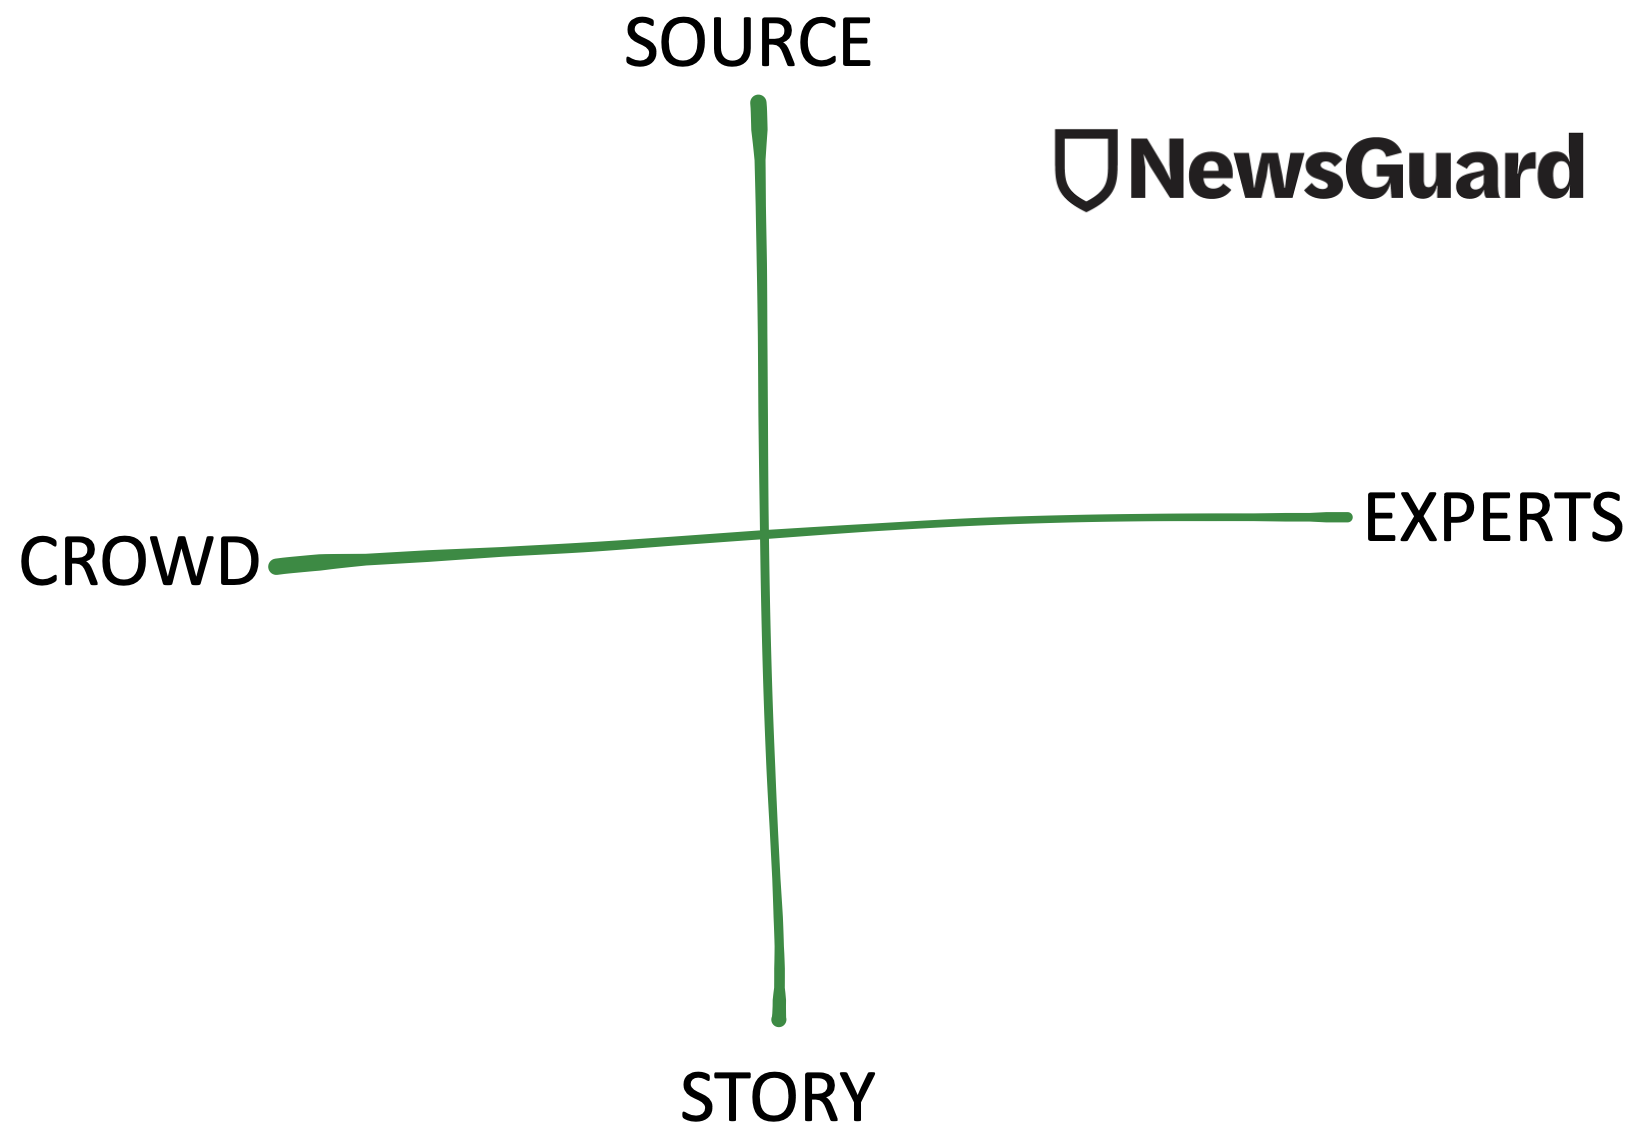
\includegraphics[width=31.25in,height=\textheight]{images/newsguard-quadrant.png}

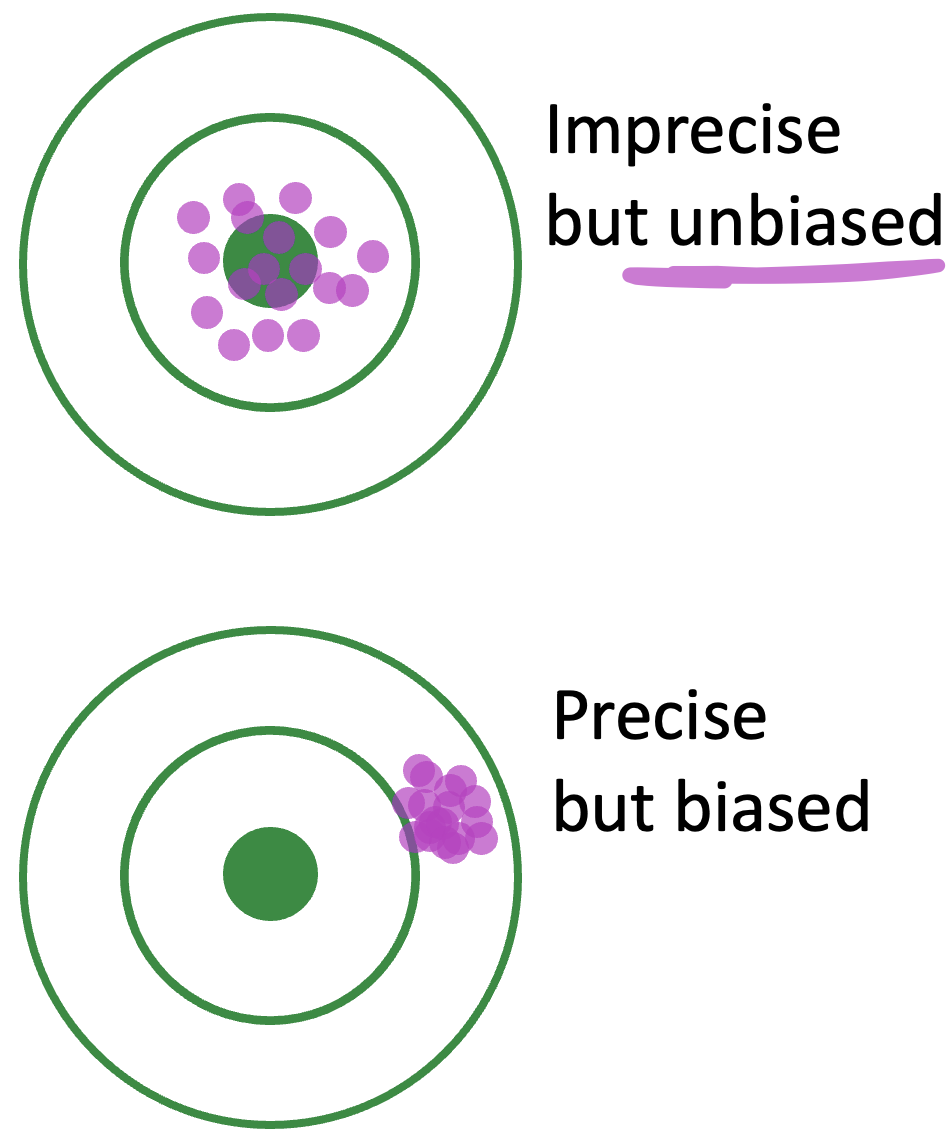
\includegraphics[width=3.125in,height=\textheight]{images/bias.png}

\(\rightarrow\) How do these choices influence downstream research
results?

Luehring, Lasser et al., (\emph{in prep.})

\begin{itemize}
\item
  When measuring misinformation, researchers have to make multiple
  decisions which majorly affect the sample
\item
  For multiple reasons, it is really hard to identify misinformation,
  leading to researchers either picking outright falsehoods as
  factchecked stories or a few bad domains compared to a few good
  domains
\item
  However, research has shown that the grey-area content may be more
  widely spread and more dangerous
\item
  If you broaden the focus on bad information to include any content
  that might be misleading even if it does not involve outright
  falsehoods and fabrications, bad information is not easy to identify -
  by misinformation researchers or anyone else
\end{itemize}

\hypertarget{problem-2}{%
\subsection{Problem \#2}\label{problem-2}}

Misinformation is measured as clearly true or false instances,

\begin{itemize}
\item
  neglecting less extreme types,
\item
  making it hard to isolate effects of misinformation.
\end{itemize}

Allen et al.,
\href{https://www.science.org/doi/10.1126/science.adk3451}{2024}; Altay
et al., \href{https://doi.org/10.1177/20563051221150412}{2023}; van der
Linden \& Krychenko,
\href{https://www.science.org/doi/10.1126/science.adp9117}{2024}

We identified two problems that we wanted to tackle in this study

\begin{itemize}
\item
  First, misinformation is often measured as clearly false, fact-checked
  instances, which ignores less extreme and more influential types of
  misinformation, for instance biased news, and it makes it hard to
  isolate the effects from real news

  \begin{itemize}
  \tightlist
  \item
    So the question is, are the effects that we are observing unique to
    misinformation?
  \end{itemize}
\item
  Second, emotions are functional; and the function of emotions hinges
  on the interaction of prior beliefs and content. Therefore, measuring
  only positive and negative sentiment, or mixing up emotional state
  with emotional reactions overlooks the contextual effects of different
  emotions.
\end{itemize}

\hypertarget{our-objectives}{%
\subsection{Our objectives}\label{our-objectives}}

\begin{enumerate}
\def\labelenumi{\arabic{enumi}.}
\tightlist
\item
  Collecting a \textbf{systematic, large-scale and long-term data set}
  for the German-speaking context
\end{enumerate}

\hypertarget{continuous-trustworthiness-ratings-by-newsguard-1}{%
\subsubsection{Continuous trustworthiness ratings by NewsGuard
(\#1)}\label{continuous-trustworthiness-ratings-by-newsguard-1}}

\begin{enumerate}
\def\labelenumi{\arabic{enumi}.}
\setcounter{enumi}{1}
\tightlist
\item
  Approximating \textbf{causal inference} to test the effects of
  misinformation on emotions
\end{enumerate}

\hypertarget{nonparametric-matching-strategy-2}{%
\subsubsection{Nonparametric matching strategy
(\#2)}\label{nonparametric-matching-strategy-2}}

So, we derived 2 major objectives:

\begin{itemize}
\item
  First, we wanted to collect a systematic, large-scale and long-term
  dataset that relies on continuous trustworthiness ratings for sources,
  including biased but relatively trustworthy sources so that it
  reflects the whole spectrum of news trustworthiness
\item
  Second, we tried a matching approach to approximate causal inference
  so that we could isolate the effects of untrustworthy sources
\end{itemize}

\hypertarget{data-collection}{%
\subsection{Data collection}\label{data-collection}}

Posts from Twitter/X mentioning any of 347 German news domains

\emph{N} = 9.3M discussions (20.6M tweets total)

93.8\% trustworthy (\textgreater60)

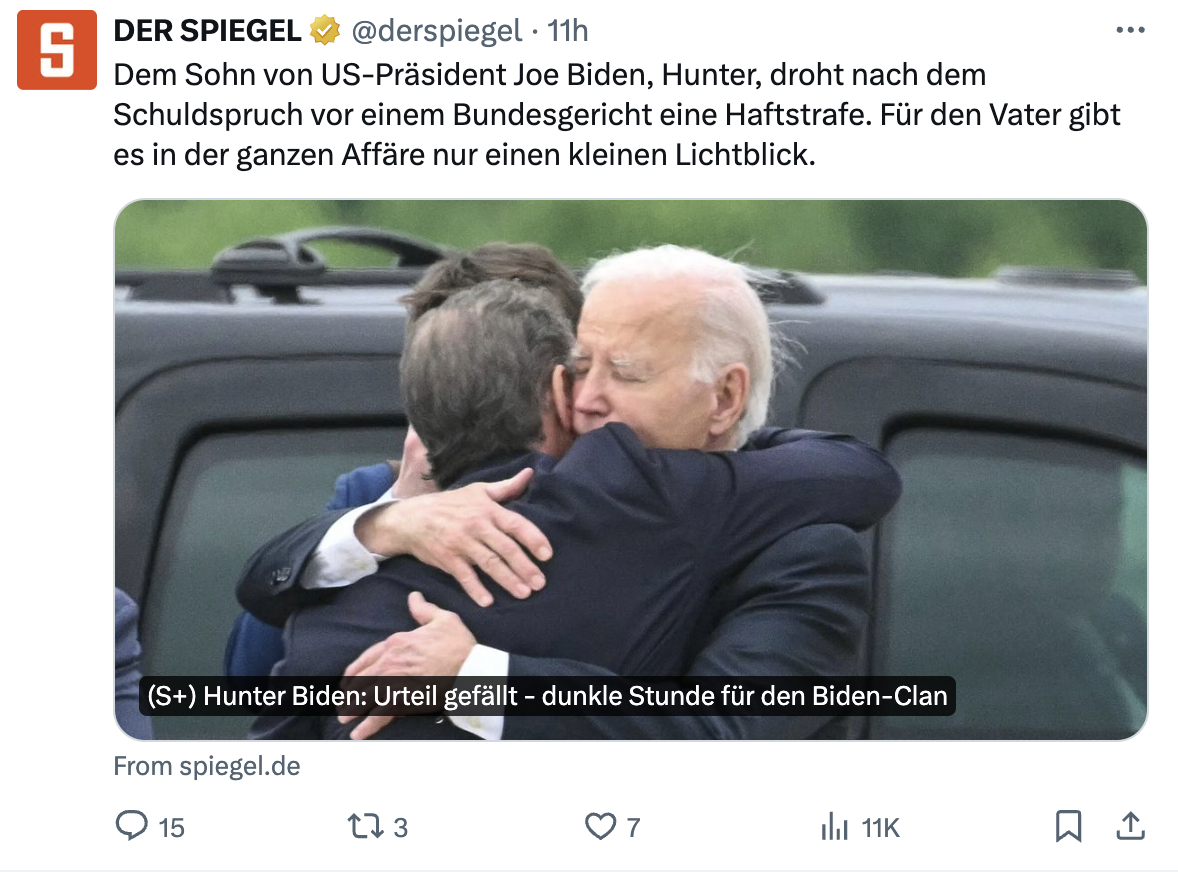
\includegraphics[width=6.25in,height=\textheight]{images/spon.png}

\hypertarget{machine-learning-classification}{%
\subsection{Machine learning
classification}\label{machine-learning-classification}}

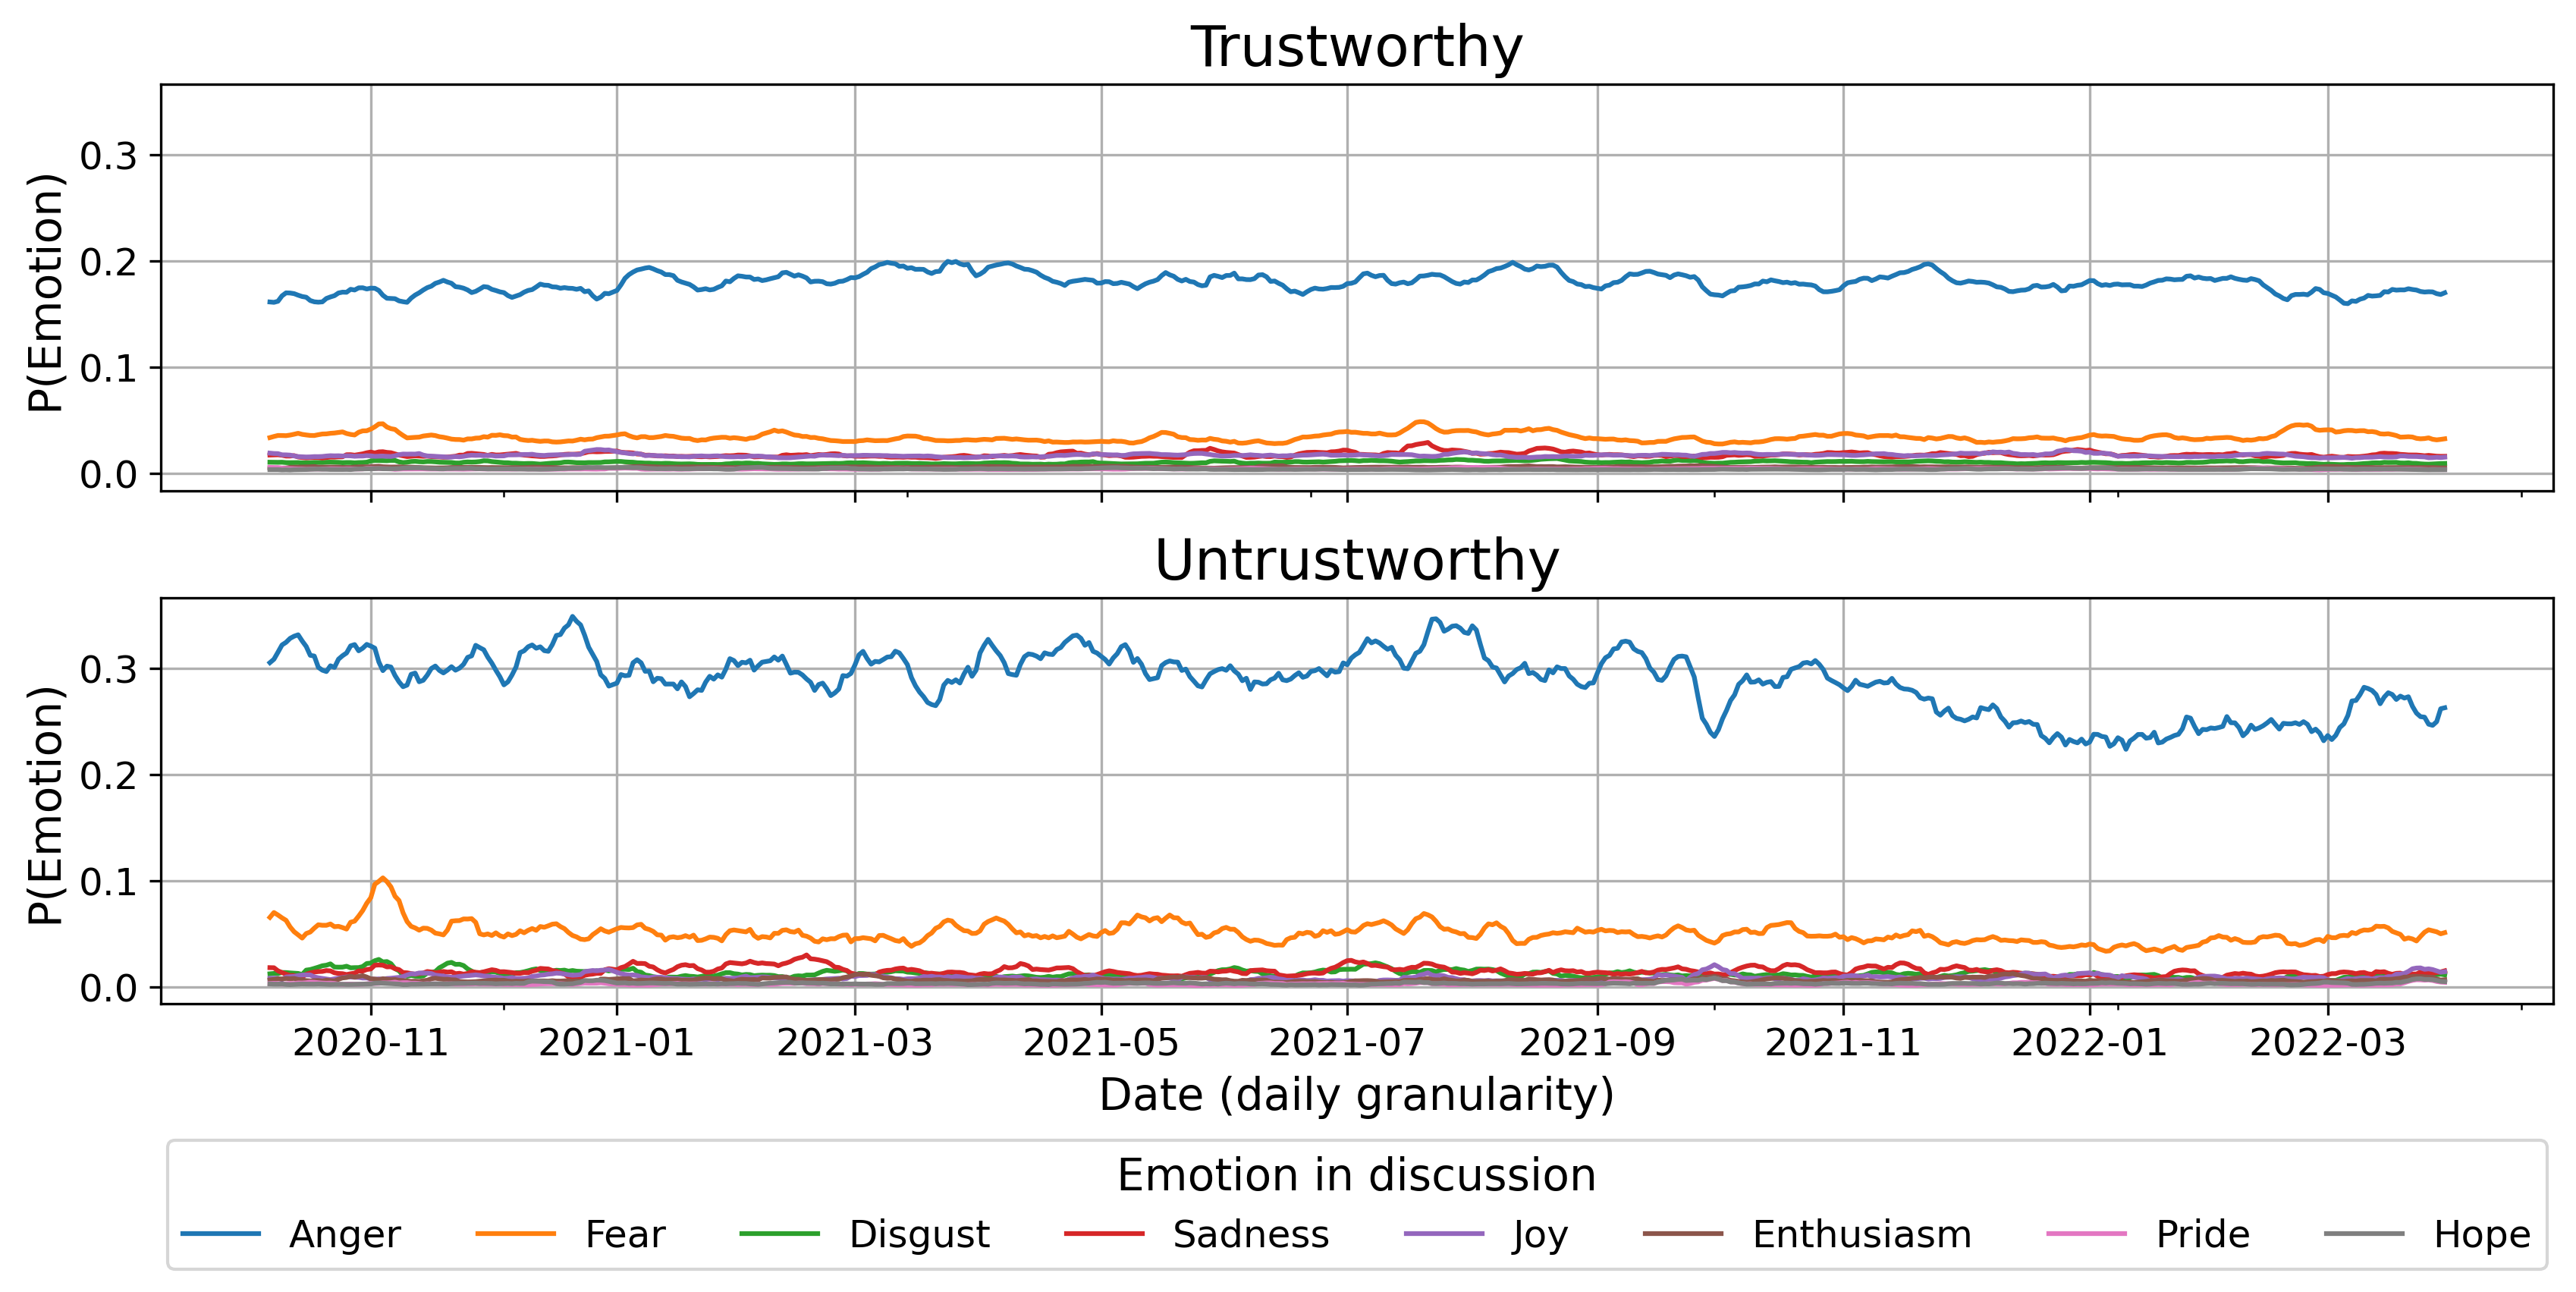
\includegraphics[width=6.25in,height=\textheight]{images/daily_emotions_rating_smoothed.png}

pol\_emo\_mDeBERTa (Widmann \& Wich,
\href{https://doi.org/10.1017/pan.2022.15}{2022}; Macro F1=0.7)

We collected roughly 9 million twitter discussions where a German news
domain was shared as the first tweet, with 20M tweets in total. For
those news domains, we have a trustworthiness rating from NewsGuard,
therefore, we understand misinformation here as news from untrustworthy
sources

\begin{itemize}
\tightlist
\item
  For each tweet, we then classified 8 distinct emotions and out-group
  references from text
\item
  This plot shows the covered time frame from October 2020 to March 2022
  and we can already see that anger is overall much higher
\end{itemize}

\hypertarget{part-i-emotion-in-the-post}{%
\section{Part I: Emotion in the post}\label{part-i-emotion-in-the-post}}

In a first step of analysis, we look at whether trustworthiness predicts
the emotion in the post

\hypertarget{is-trustworthiness-associated-with-anger}{%
\subsection{Is trustworthiness associated with
anger?}\label{is-trustworthiness-associated-with-anger}}

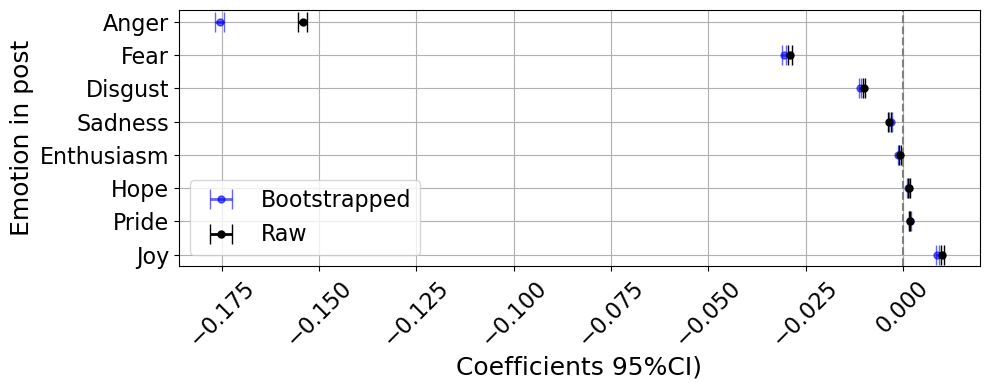
\includegraphics[width=6.25in,height=\textheight]{images/emo_in_post_coeff_boot.png}

\(\rightarrow\) Trustworthiness predicts a 15\% decrease in anger

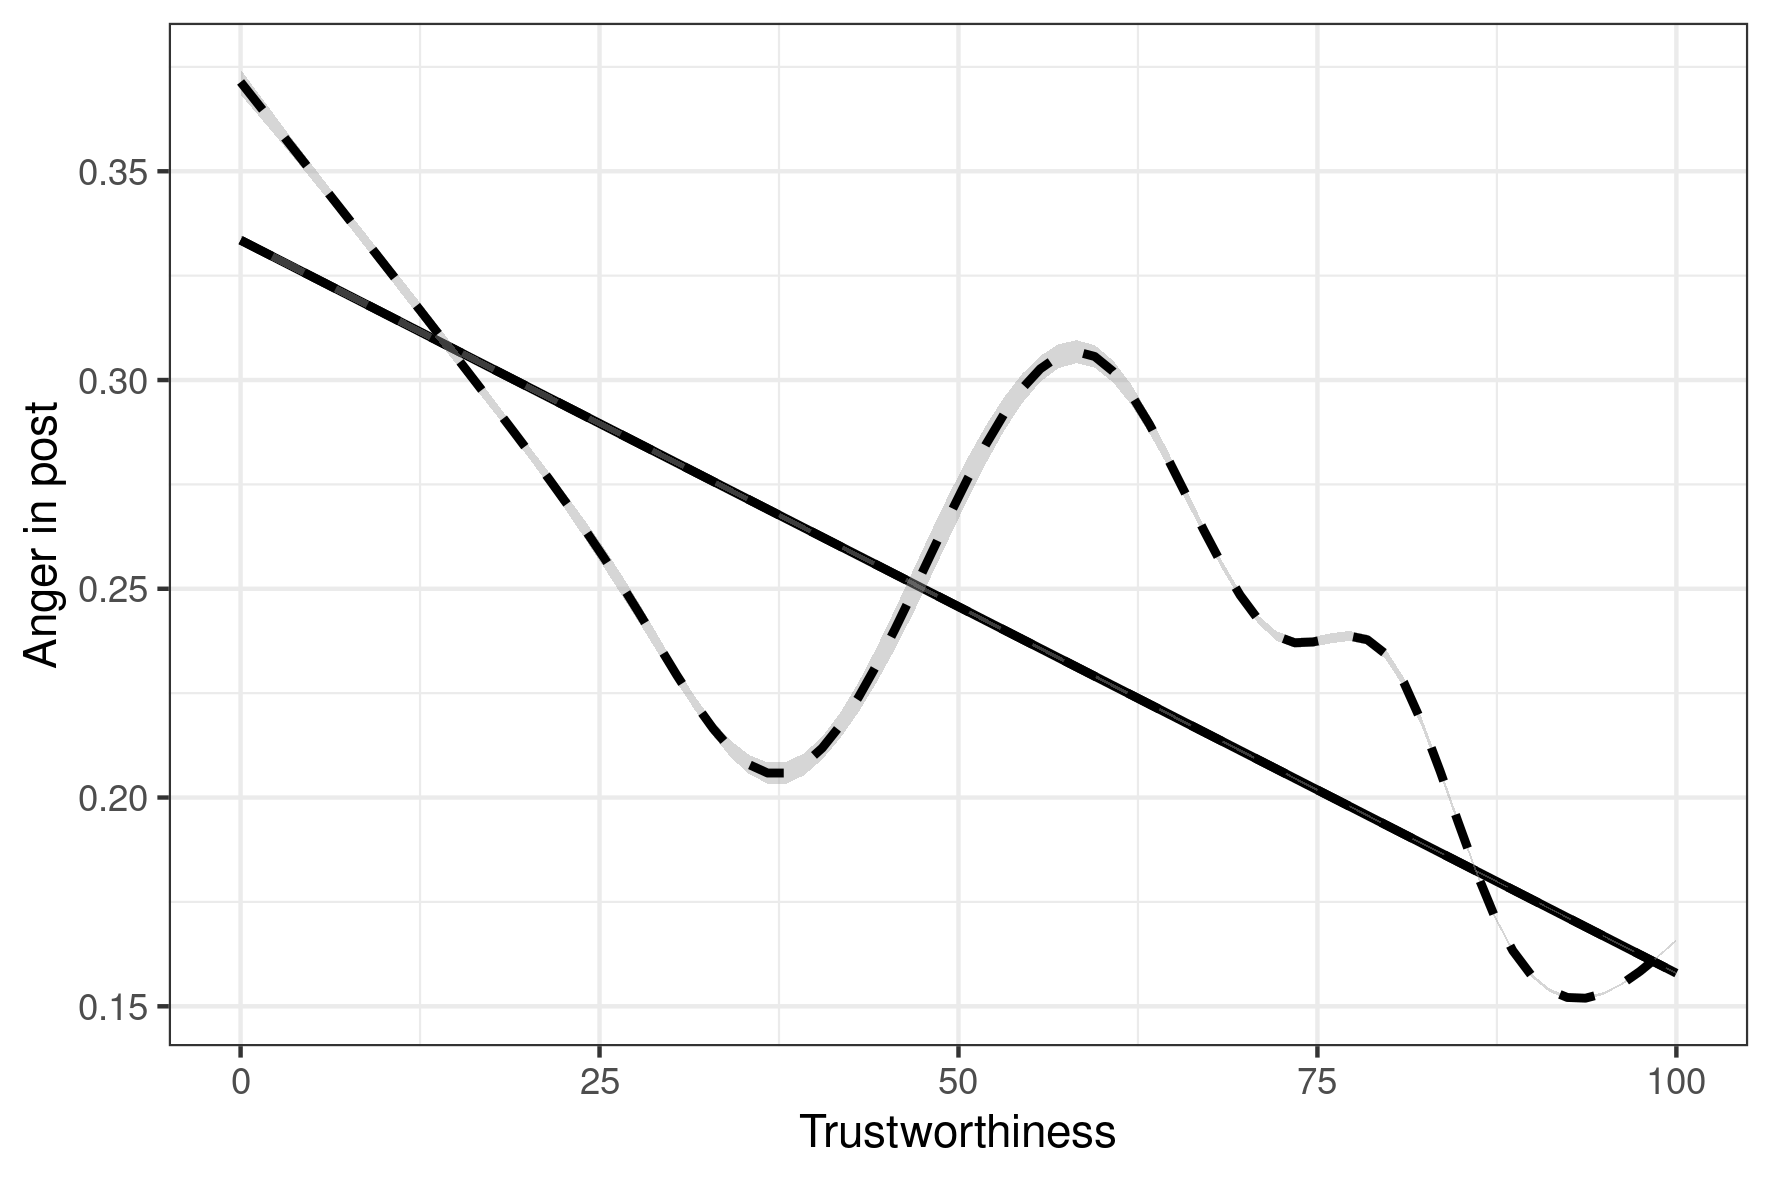
\includegraphics[width=10.41667in,height=\textheight]{images/anger_score_loess.png}

But gray-area content matters, too!

We especially wanted to see if tweets with a lower trustworthiness score
also included more anger

And that's also what we found!

Anger decreases when trustworthiness increases

While joy increases when trustworthiness increases

\hypertarget{part-ii-engagement}{%
\section{Part II: Engagement}\label{part-ii-engagement}}

\hypertarget{is-lower-trustworthiness-associated-with-higher-engagement}{%
\subsection{Is lower trustworthiness associated with higher
engagement?}\label{is-lower-trustworthiness-associated-with-higher-engagement}}

\textsubscript{Models:~Zero-inflated~Negative~Binomial~(log-link)}

\textsubscript{Controls:~PO,~word~count,~following,~initial~emotions}

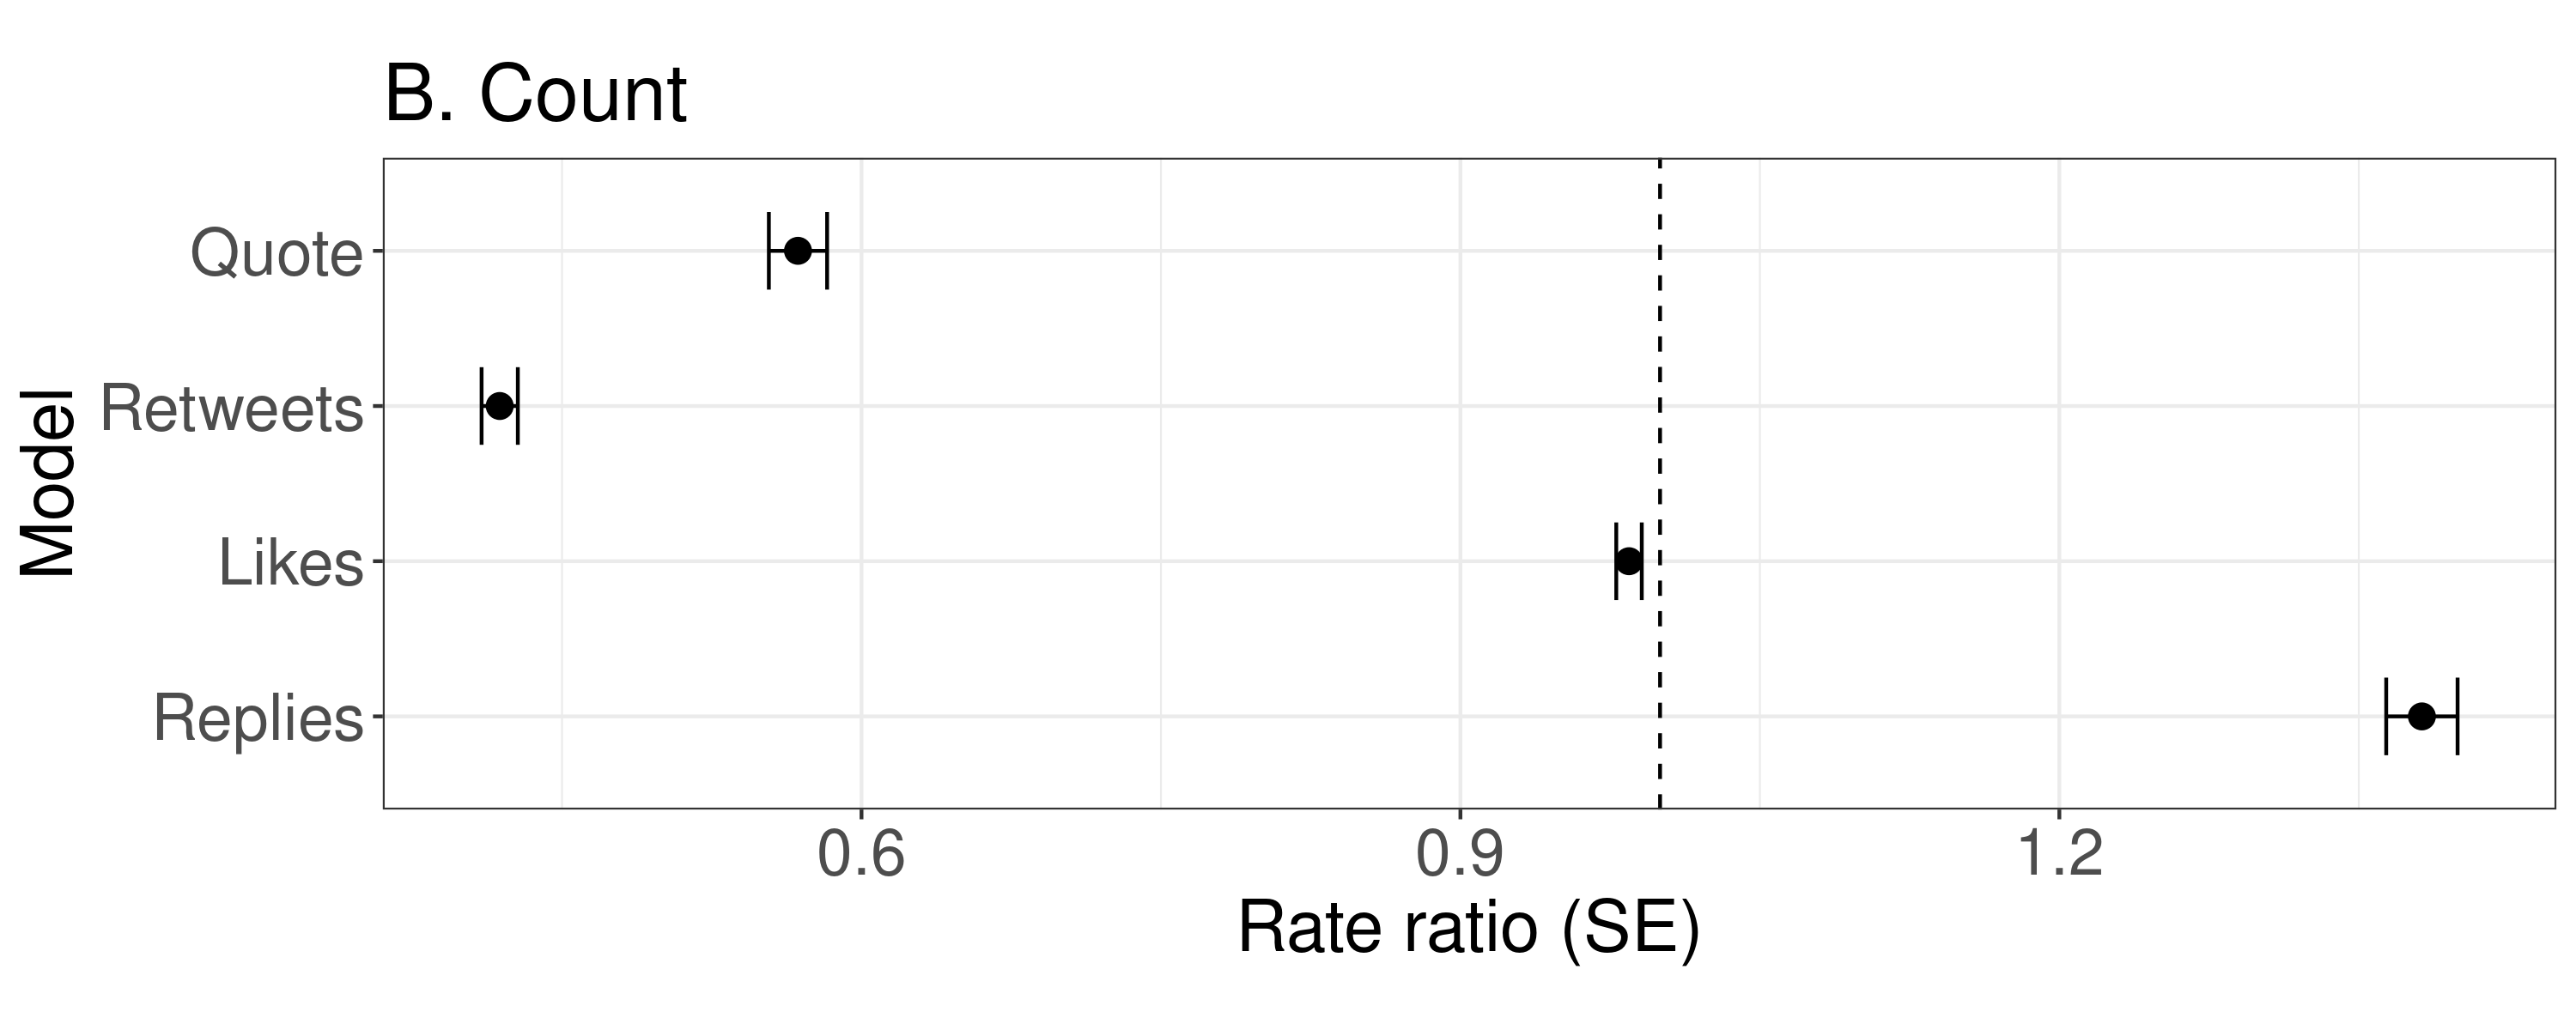
\includegraphics[width=6.25in,height=\textheight]{images/models_zinb_estimates-se.png}

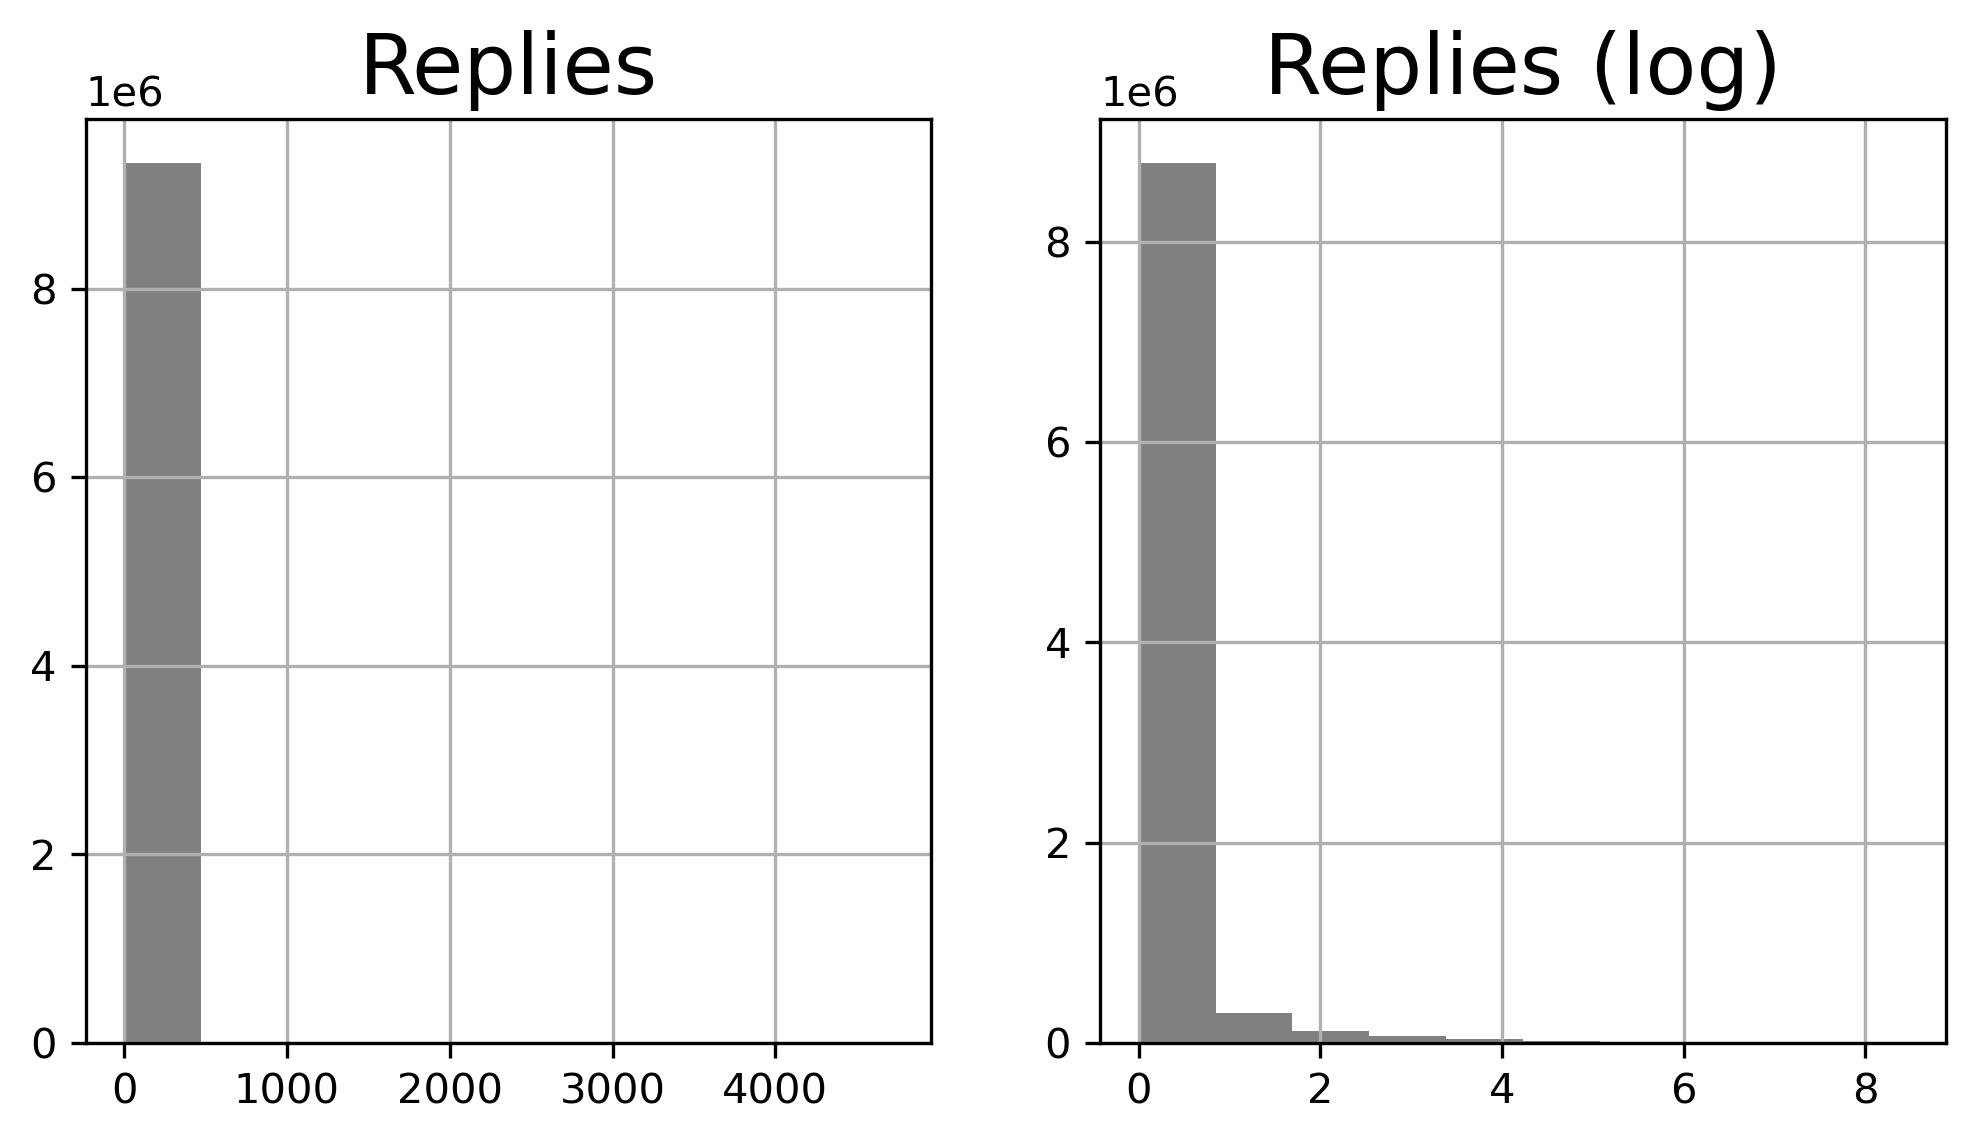
\includegraphics[width=3.125in,height=\textheight]{images/reply_distributions.png}

\(\rightarrow\) 58\% decrease in retweets and 43\% decrease in quotes

Zeileis et al., \href{http://www.jstatsoft.org/v27/i08/}{2008}

Lastly, we wanted to look at the associations between trustworthiness
and engagement

Here, we included the zero replies, which zero-inflated the
distribution, which you can see in the top corner

\begin{itemize}
\item
  The results of our logistic regression model show that trustworthy
  information generally gets more likes than untrustworthy information.
  And the count model shows that, when excess zeroes are excluded, a
  lower trustworthiness score is associated with more retweets and quote
  retweets
\item
  Bad sources getting more reshares is also in line with the FB and
  Instagram experiments, where removing reshares reduced the exposure to
  misinformation.
\end{itemize}

\hypertarget{part-iii-emotional-responses}{%
\section{Part III: Emotional
responses}\label{part-iii-emotional-responses}}

\hypertarget{a-correlations}{%
\section{A) Correlations}\label{a-correlations}}

\hypertarget{emotional-response-reflects-emotion-in-post}{%
\subsection{Emotional response reflects emotion in
post}\label{emotional-response-reflects-emotion-in-post}}

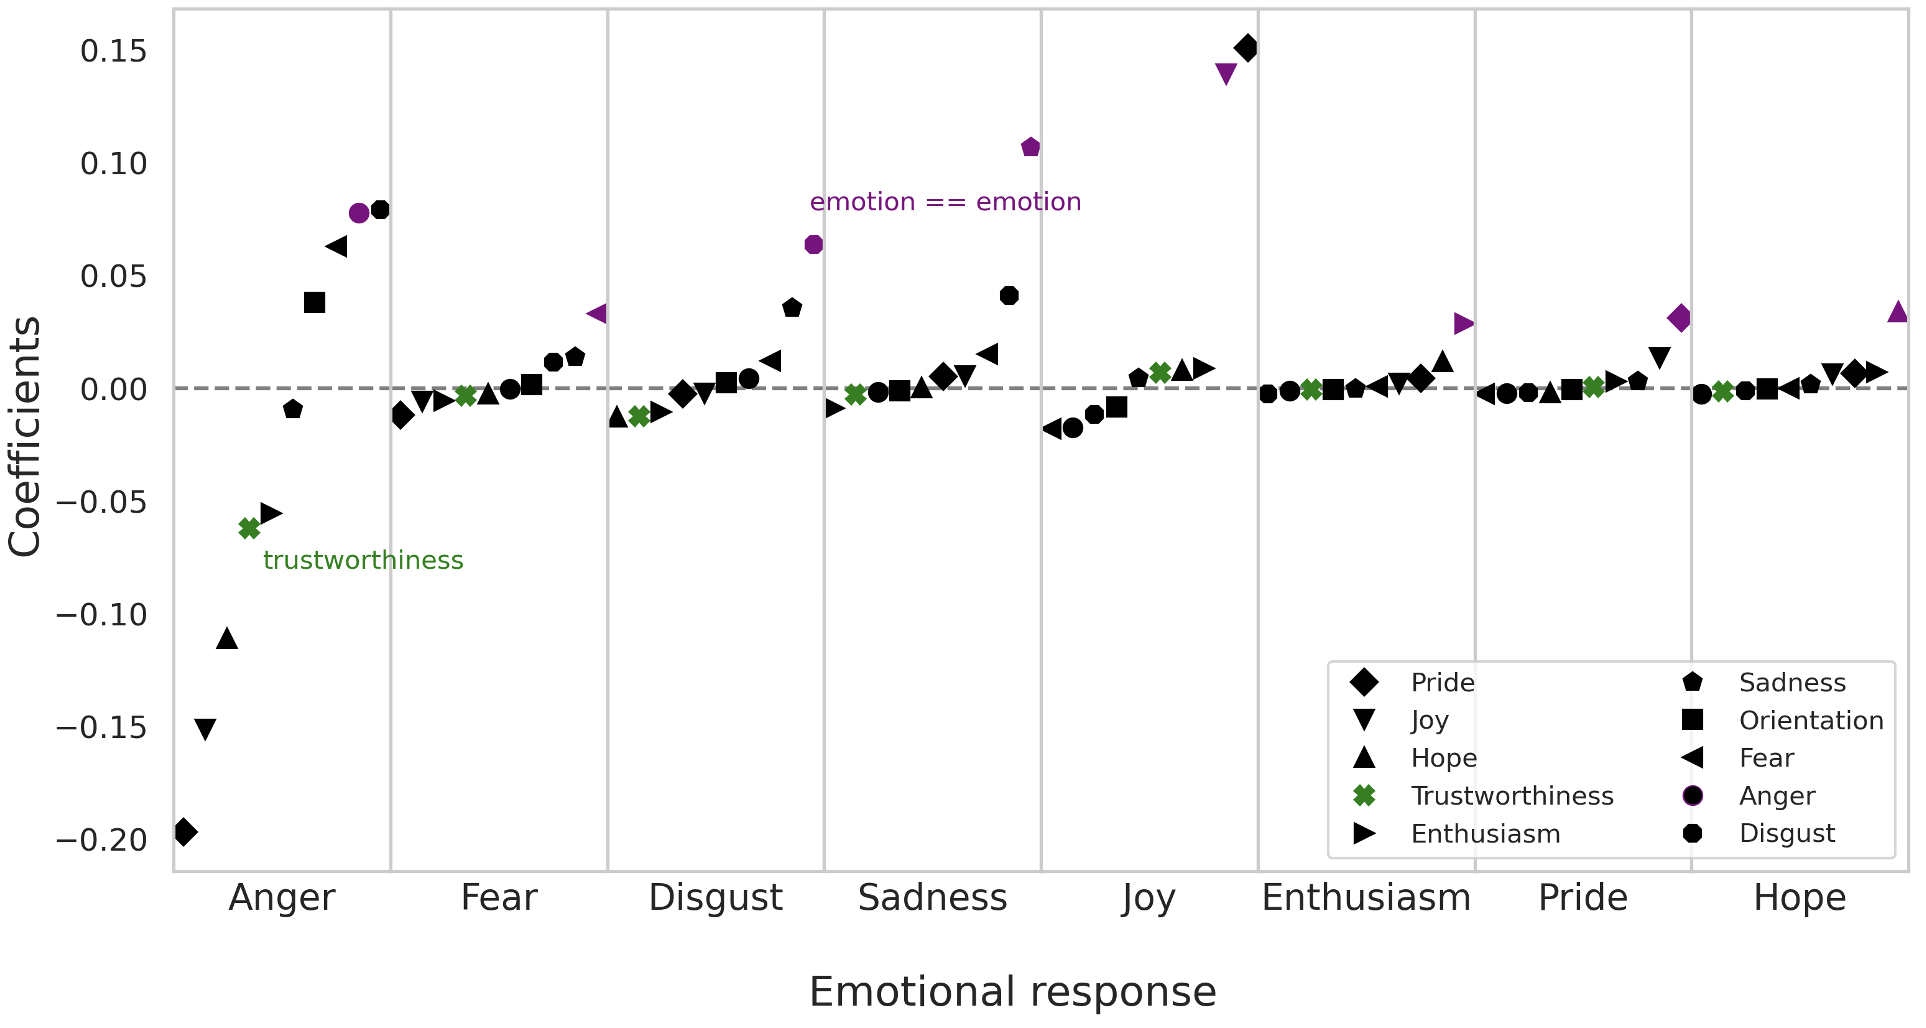
\includegraphics[width=9.375in,height=\textheight]{images/emo_coeffs.png}

\(\rightarrow\) Does trustworthiness actually affect emotional
reactions?

\hypertarget{b-causal-inference}{%
\section{B) Causal inference}\label{b-causal-inference}}

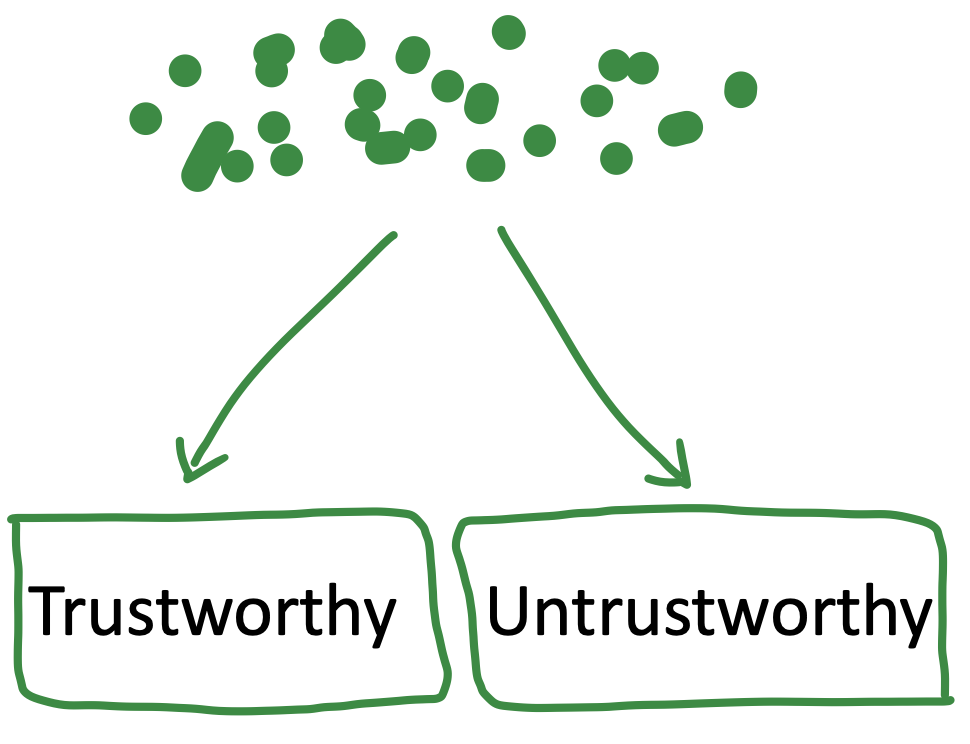
\includegraphics[width=3.125in,height=\textheight]{images/randomization.png}

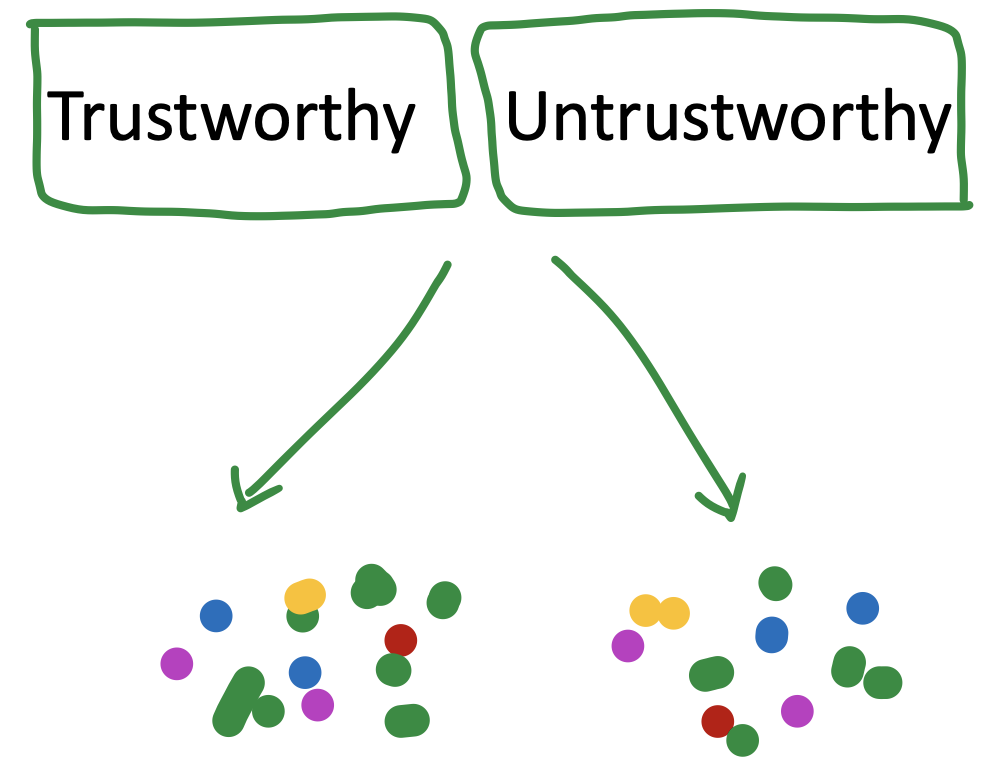
\includegraphics[width=3.125in,height=\textheight]{images/matching.png}

Now, we are zooming in on the tweets that got at least one reply and the
following discussion thread

\hypertarget{nonparametric-matching}{%
\subsection{Nonparametric matching}\label{nonparametric-matching}}

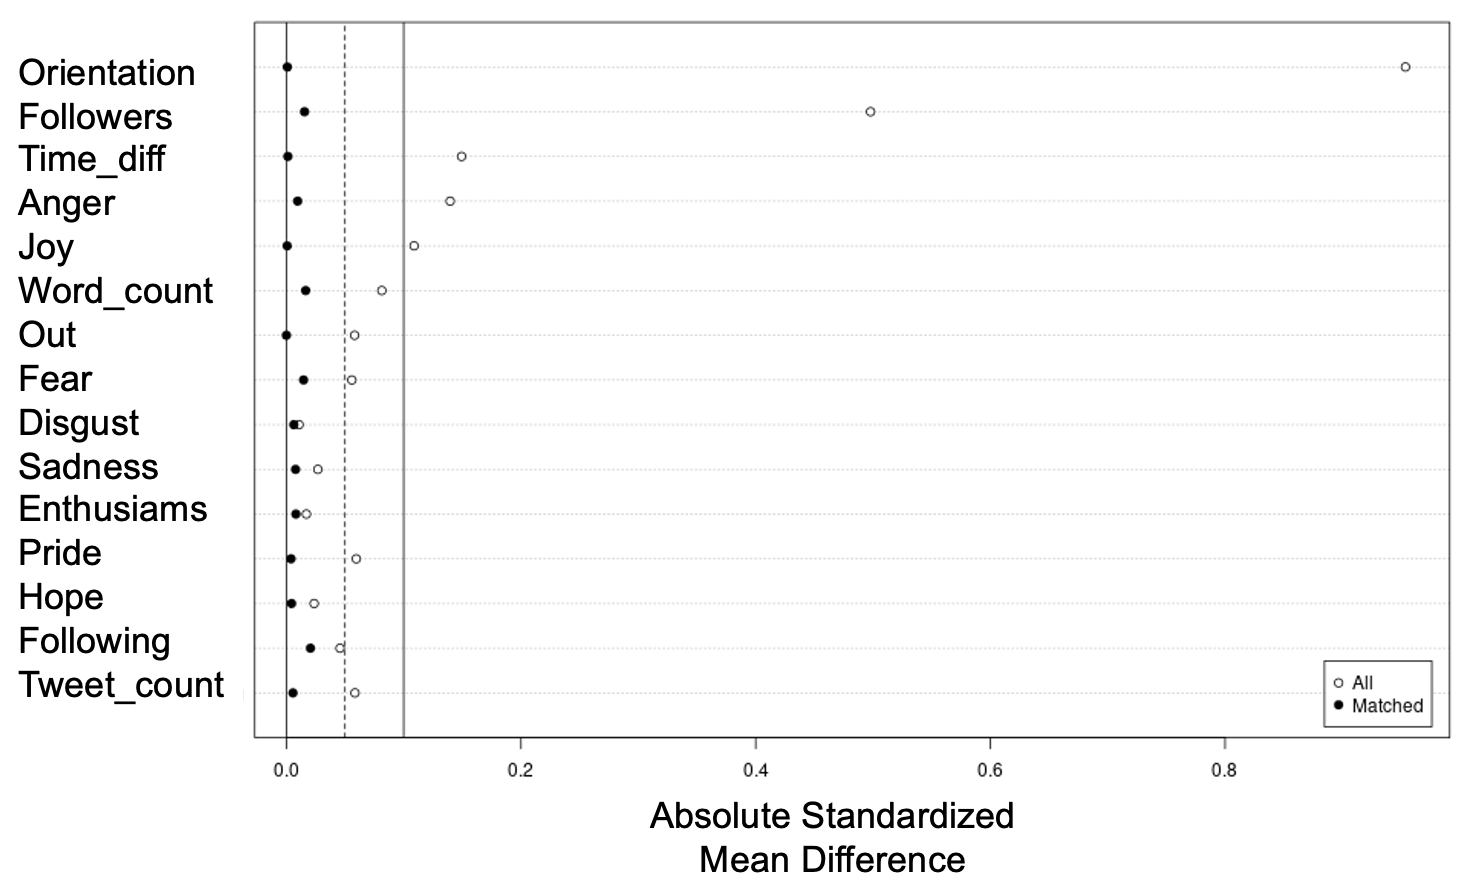
\includegraphics[width=7.29167in,height=\textheight]{images/mahalanobis_plot_wd.png}

Nearest Neighbor and Mahalanobis distance

\(\rightarrow\) \emph{N} = 87,132

Ho et al.,
\href{https://www.cambridge.org/core/journals/political-analysis/article/matching-as-nonparametric-preprocessing-for-reducing-model-dependence-in-parametric-causal-inference/4D7E6D07C9727F5A604E5C9FCCA2DD21}{2007}

NewsGuard sets a threshold at a trustworthiness score at 60, such that
sources below 60 are considered untrustworthy

We used this classification to create two conditions (trustworthy vs
untrustworthy) and then applied a nonparametric matching approach to
balance the dataset based on a set of covariates

Those are the political orientation of the source, the initial emotion
in the tweet, following, follower and tweet counts, as well as the word
count of the first tweet

We also included the time difference between the first reply and the
last to control for collective emotional development

This plot shows the initial standardized mean difference between the two
conditions in white dots and the balanced data in black, where we can
see that by matching fitting cases, we reduced it to almost 0 for most
covariates, so we literally hold them constant across the two conditions

This approach reduced the balanced dataset to 87,000 discussions

\hypertarget{does-trustworthiness-affect-emotional-responses}{%
\subsection{Does trustworthiness affect emotional
responses?}\label{does-trustworthiness-affect-emotional-responses}}

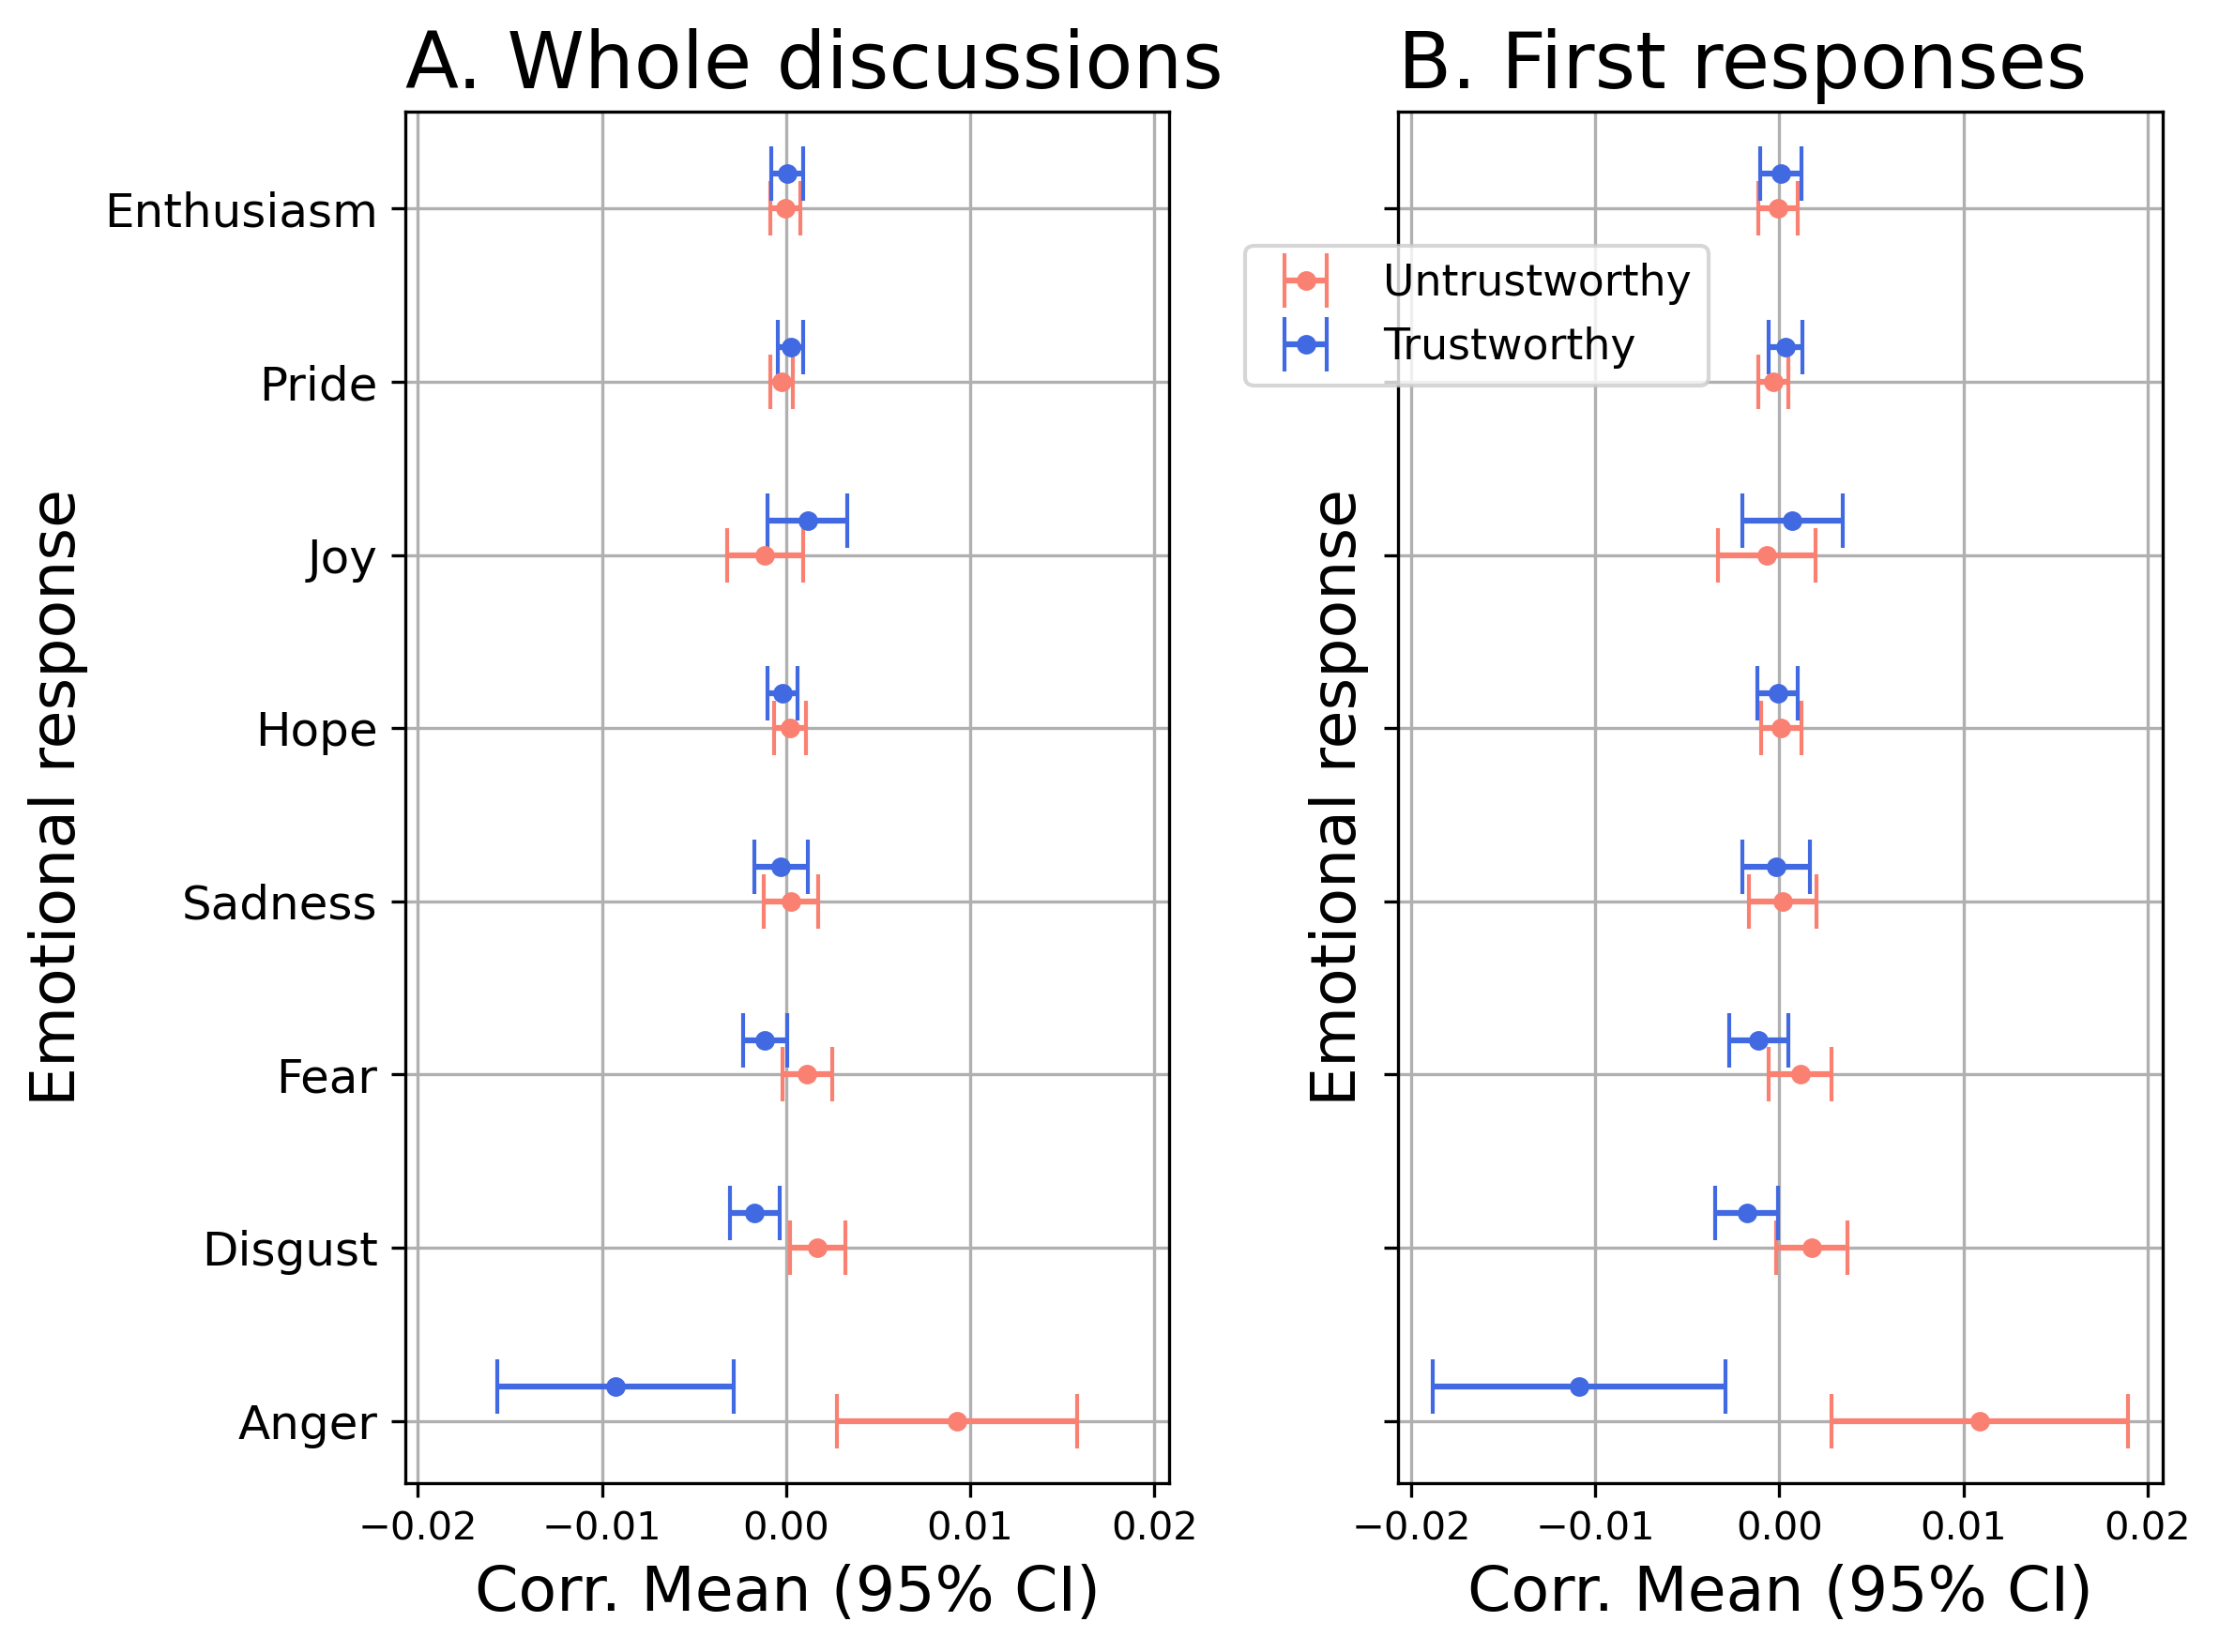
\includegraphics[width=8.33333in,height=\textheight]{images/mean_emotion_matched-95.png}

\(\rightarrow\) Less joy

\(\rightarrow\) 2\% more anger

TBD: responses within-users (responding to trustworthy and untrustworthy
posts), see Carrella et al., \href{https://osf.io/qx34w}{2023}

So, do emotions differ based on trustworthiness?

Here, we can see the mean differences in emotions between trustworthy vs
untrustworthy discussion threads, with emotions measured in both the
whole discussion aggregated and only the first response to the stimuli

\begin{itemize}
\tightlist
\item
  In both, there are significant differences in most emotions, except
  for enthusiasm, however, we observe substantially more anger, more
  out-group references and less joy in response to untrustworthy
  information
\end{itemize}

\hypertarget{c-direction-of-anger-tbd}{%
\subsection{C) Direction of anger
(TBD)}\label{c-direction-of-anger-tbd}}

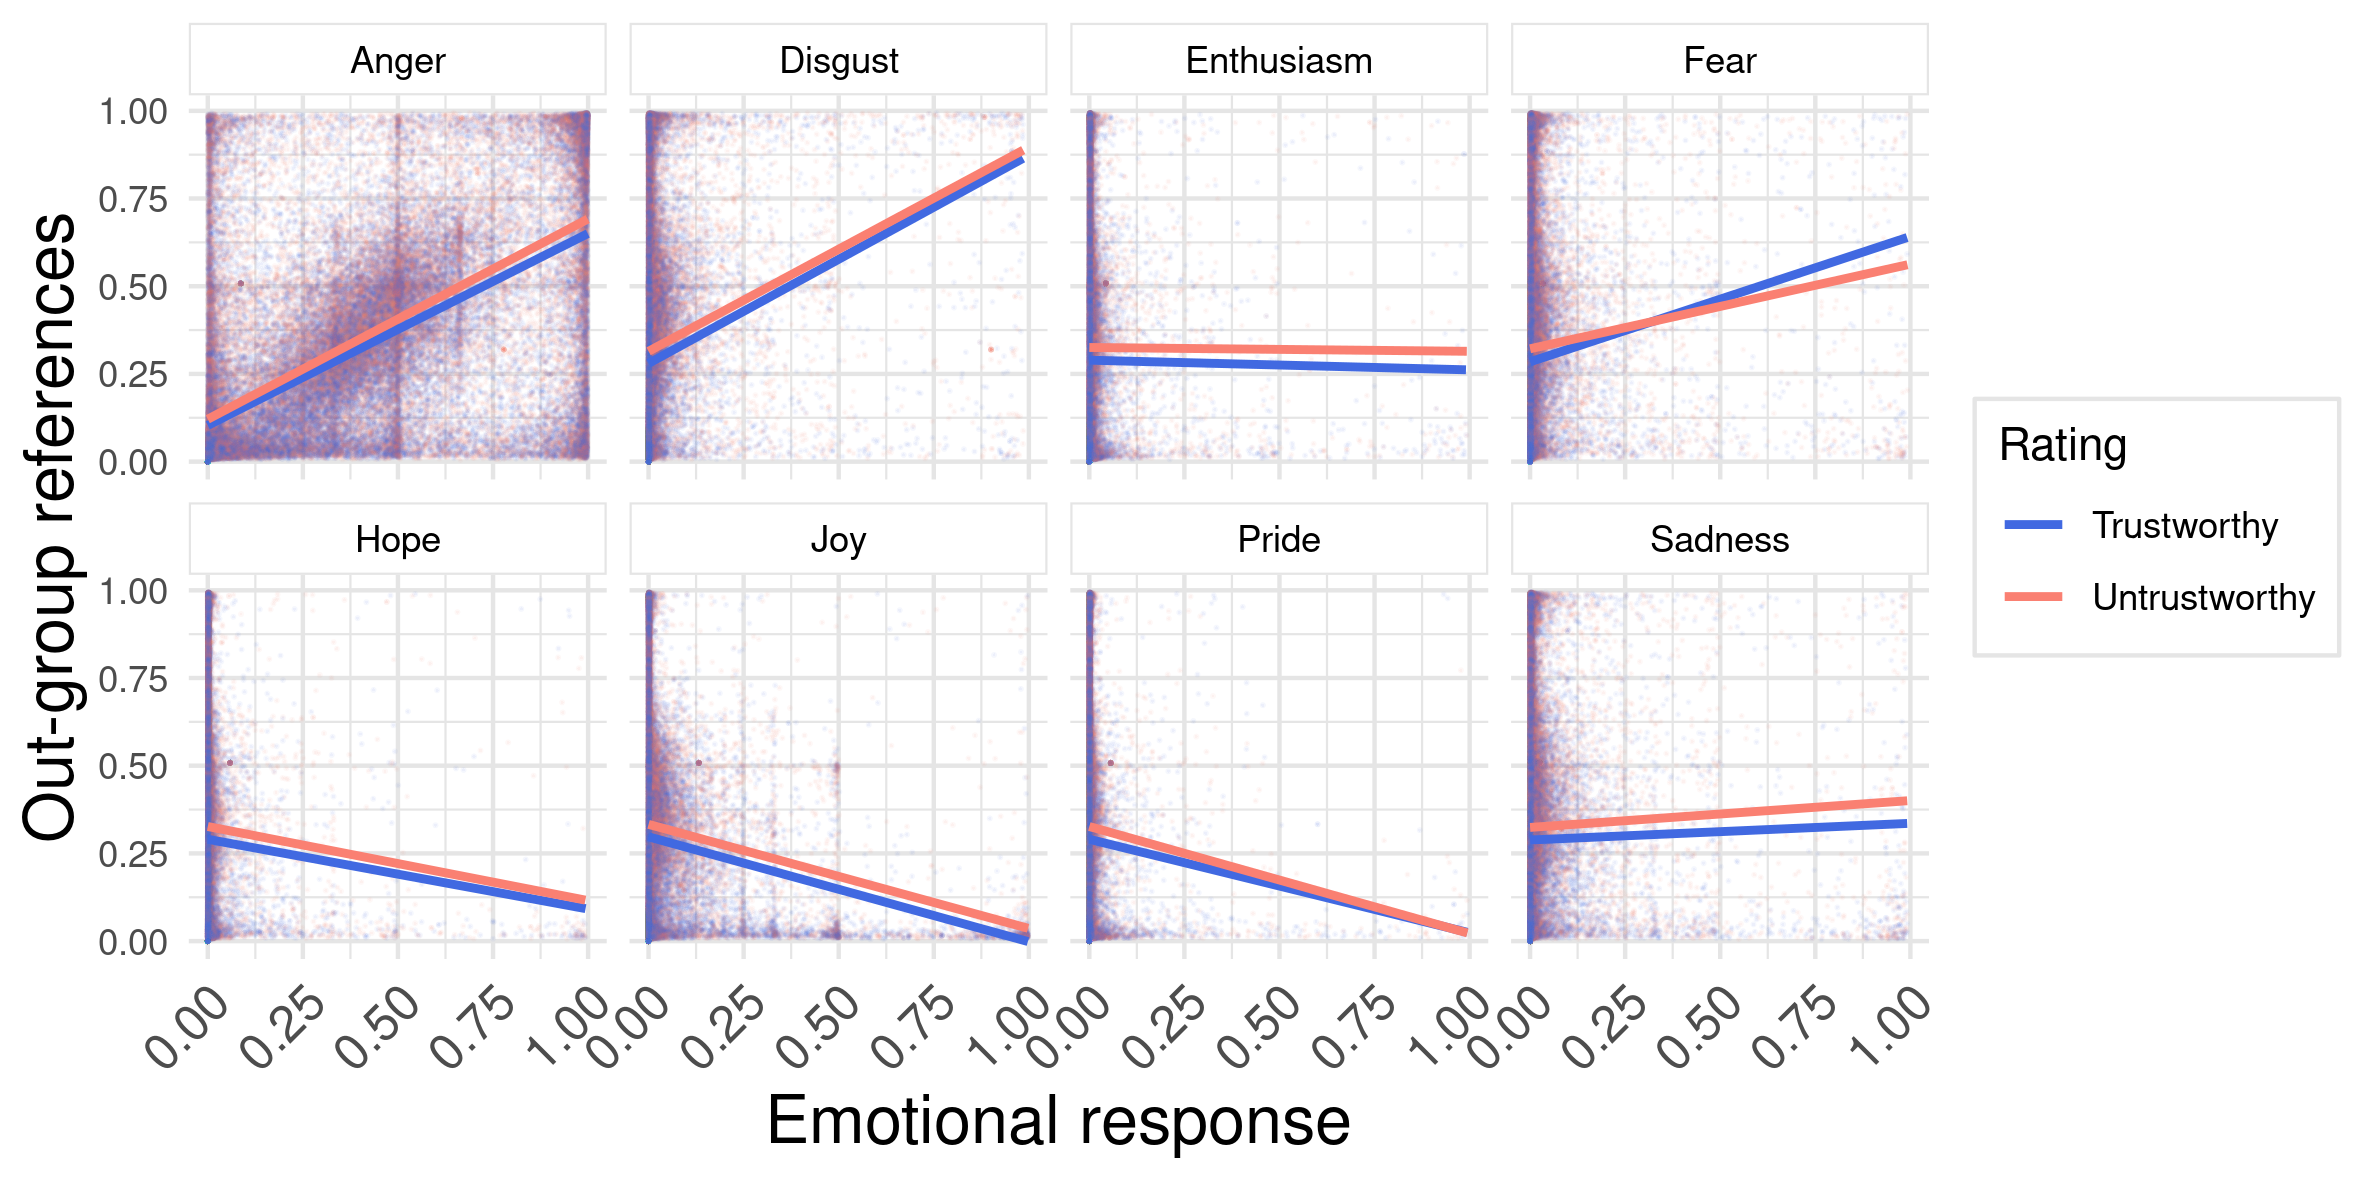
\includegraphics[width=20.83333in,height=\textheight]{images/emotion_outgroup_facet.png}
Out-group classification (Lasser at al., 2023; F1=0.8)

\hypertarget{c-origin-of-anger-tbd}{%
\subsection{C) Origin of anger (TBD)}\label{c-origin-of-anger-tbd}}

\begin{itemize}
\tightlist
\item
  How do people talk in most angry discussions? Do they counterargue?
\end{itemize}

\begin{itemize}
\item
  What are the topics in the first post?
\item
  Do the discussion networks differ (see Gonzalez-Bailon et al.,
  \href{https://doi.org/10.1057/jit.2010.2}{2010})?
\end{itemize}

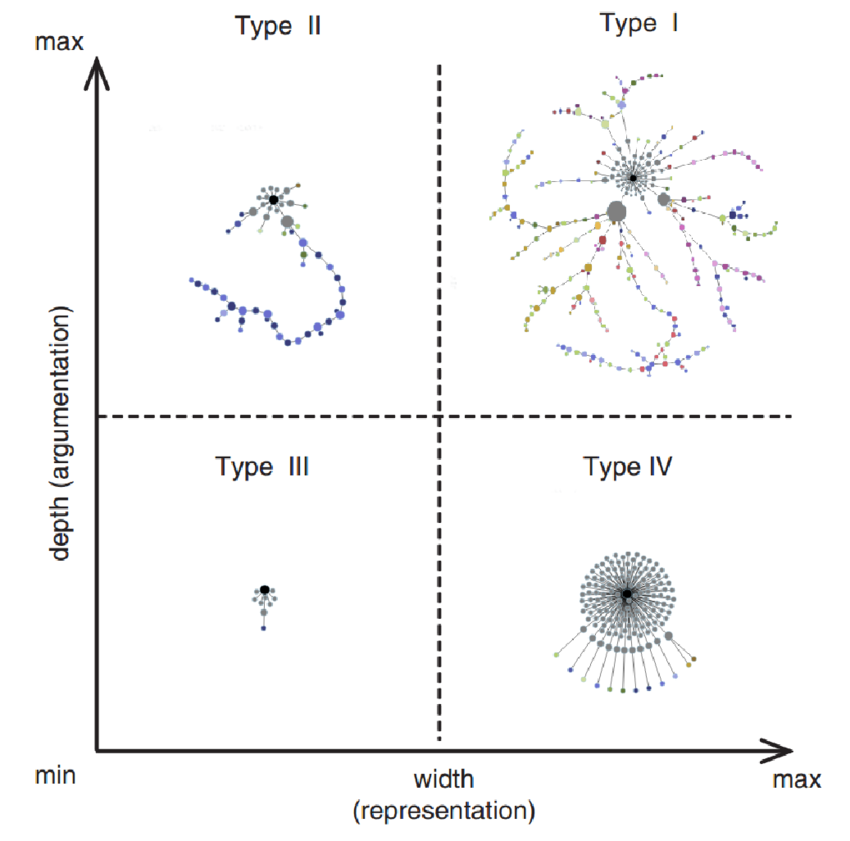
\includegraphics[width=7.29167in,height=\textheight]{images/four-types-of-discussions.png}

\hypertarget{conclusion-tentative}{%
\section{Conclusion (tentative)}\label{conclusion-tentative}}

\hypertarget{emotions-rightarrow-emotions-rightarrow-engagement}{%
\subsection{\texorpdfstring{Emotions \(\rightarrow\) emotions
\(\rightarrow\)
engagement?}{Emotions \textbackslash rightarrow emotions \textbackslash rightarrow engagement?}}\label{emotions-rightarrow-emotions-rightarrow-engagement}}

\begin{itemize}
\tightlist
\item
  Sources with low trustworthiness predict anger
\item
  Emotions in discussions largely reflect emotions in initial post
\item
  Is engagement with low trustworthiness due to other factors?
\end{itemize}

\(\rightarrow\) Not the factfulness is harmful, but the content

\(\rightarrow\) Misinformation is a perfect tool to spread hateful
content

\begin{itemize}
\tightlist
\item
  Low trustworthiness predicts anger and conflict in discussions
\item
  But, emotions in discussions largely reflect emotions in initial posts
\item
  Therefore, we assume that misinformation includes more anger and
  conflict, which leads to engagement, not the trustworthiness. If we
  measured topics, this effect would probably largely be explained by
  that.
\end{itemize}

\hypertarget{thank-you}{%
\section{Thank you!}\label{thank-you}}

Email: \url{jula.luehring@univie.ac.at}

Bluesky:
\href{https://bsky.app/profile/julaluehring.bsky.social}{@julaluehring.bsky.social}

X: \href{https://twitter.com/lue_jula}{@lue\_jula}


\includegraphics[width=6.25in,height=\textheight]{logos/logos-combined.png}


\includegraphics[width=6.25in,height=\textheight]{images/frame.png}

\hypertarget{is-lower-trustworthiness-associated-with-higher-engagement-1}{%
\subsection{Is lower trustworthiness associated with higher
engagement?}\label{is-lower-trustworthiness-associated-with-higher-engagement-1}}

\textsubscript{Models:~Zero-inflated~Negative~Binomial~(log-link)}

\textsubscript{Controls:~PO,~word~count,~following,~initial~emotions}

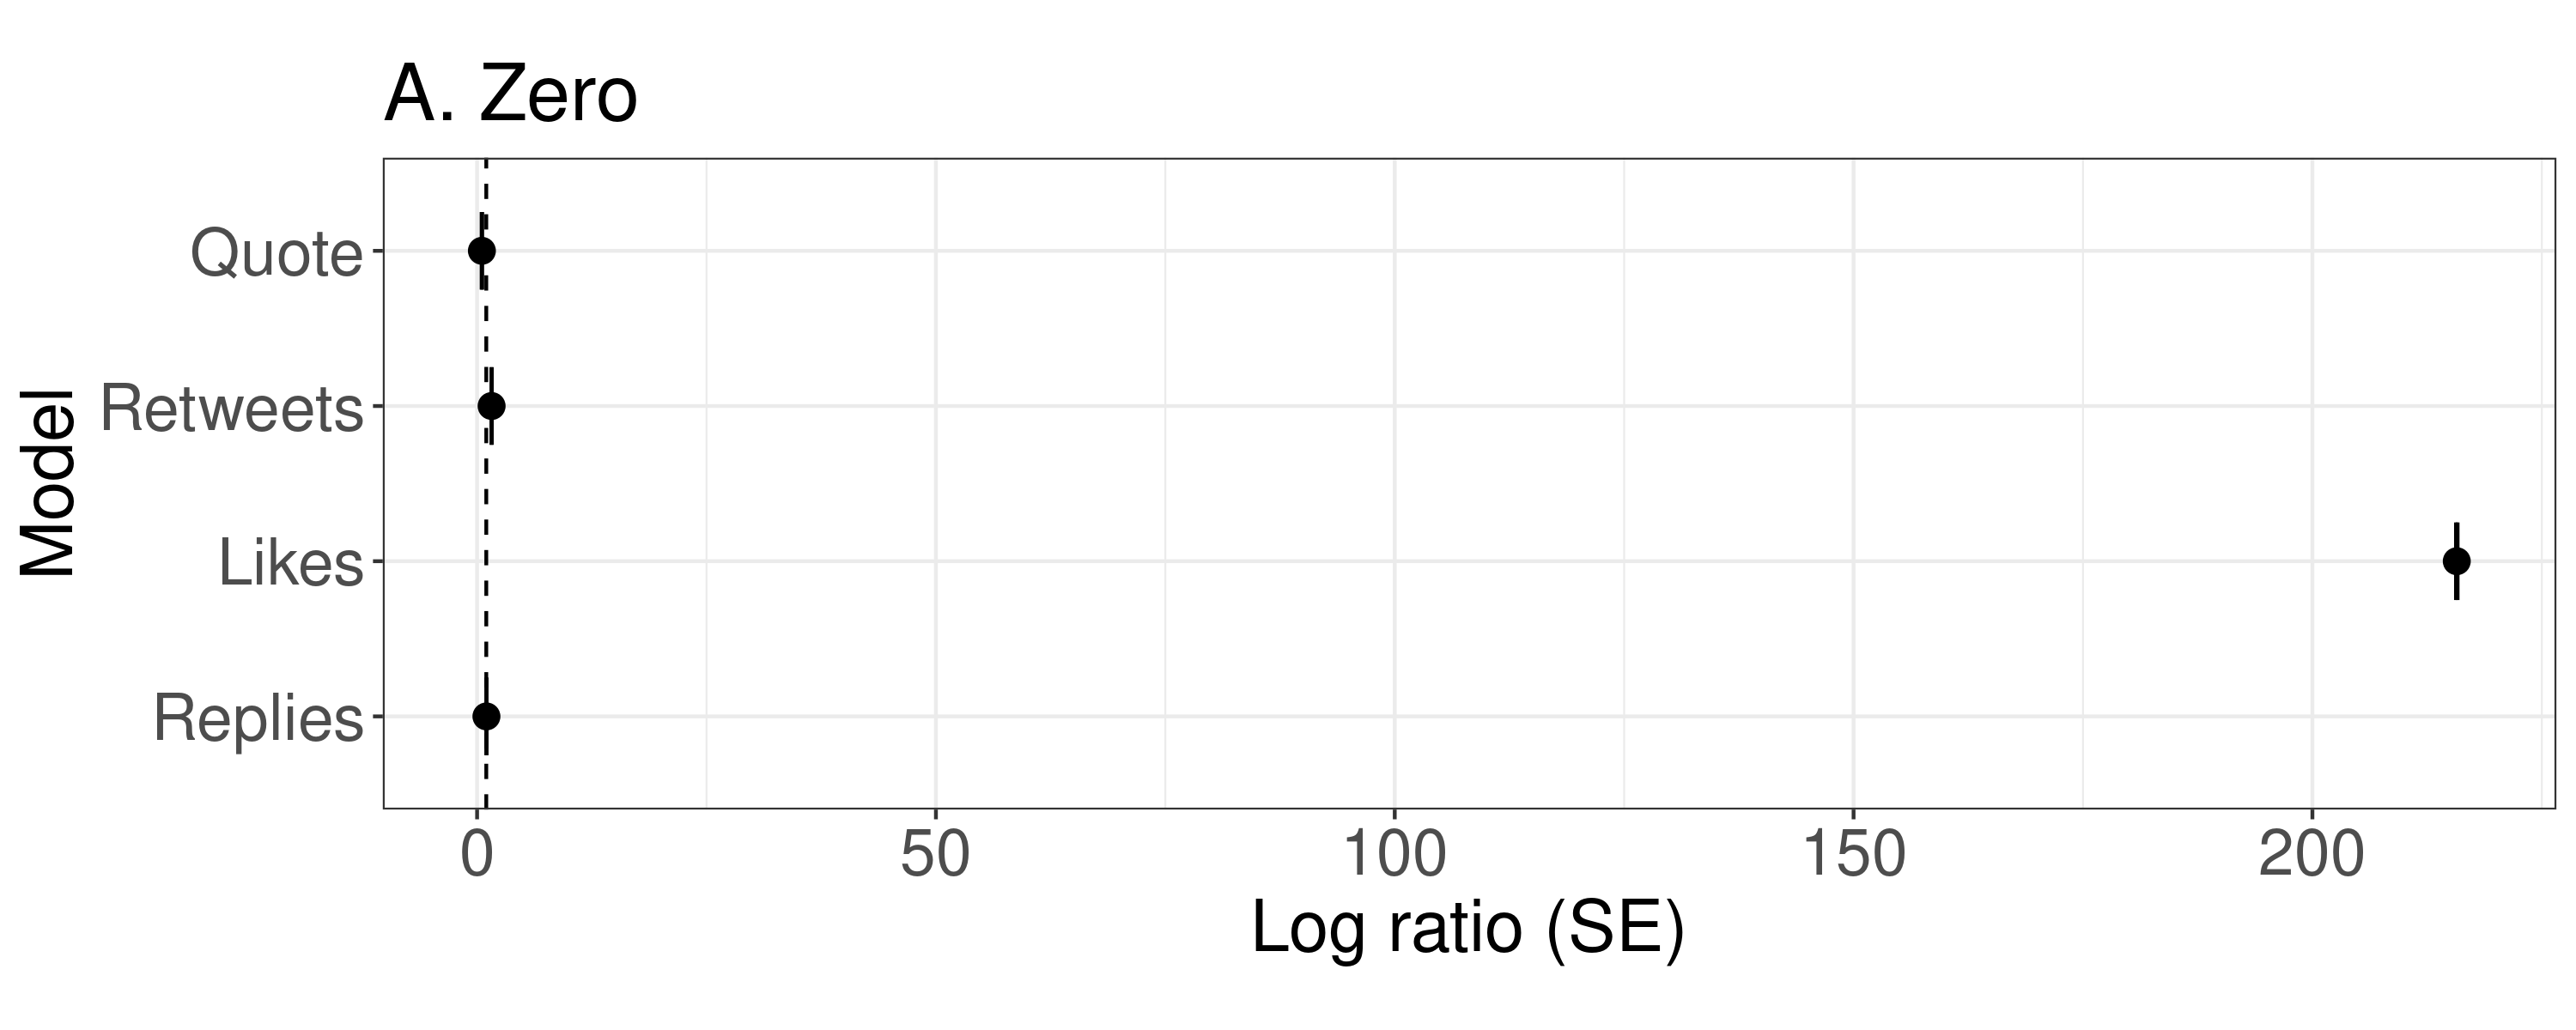
\includegraphics[width=6.25in,height=\textheight]{images/models_zero_estimates-se.png}

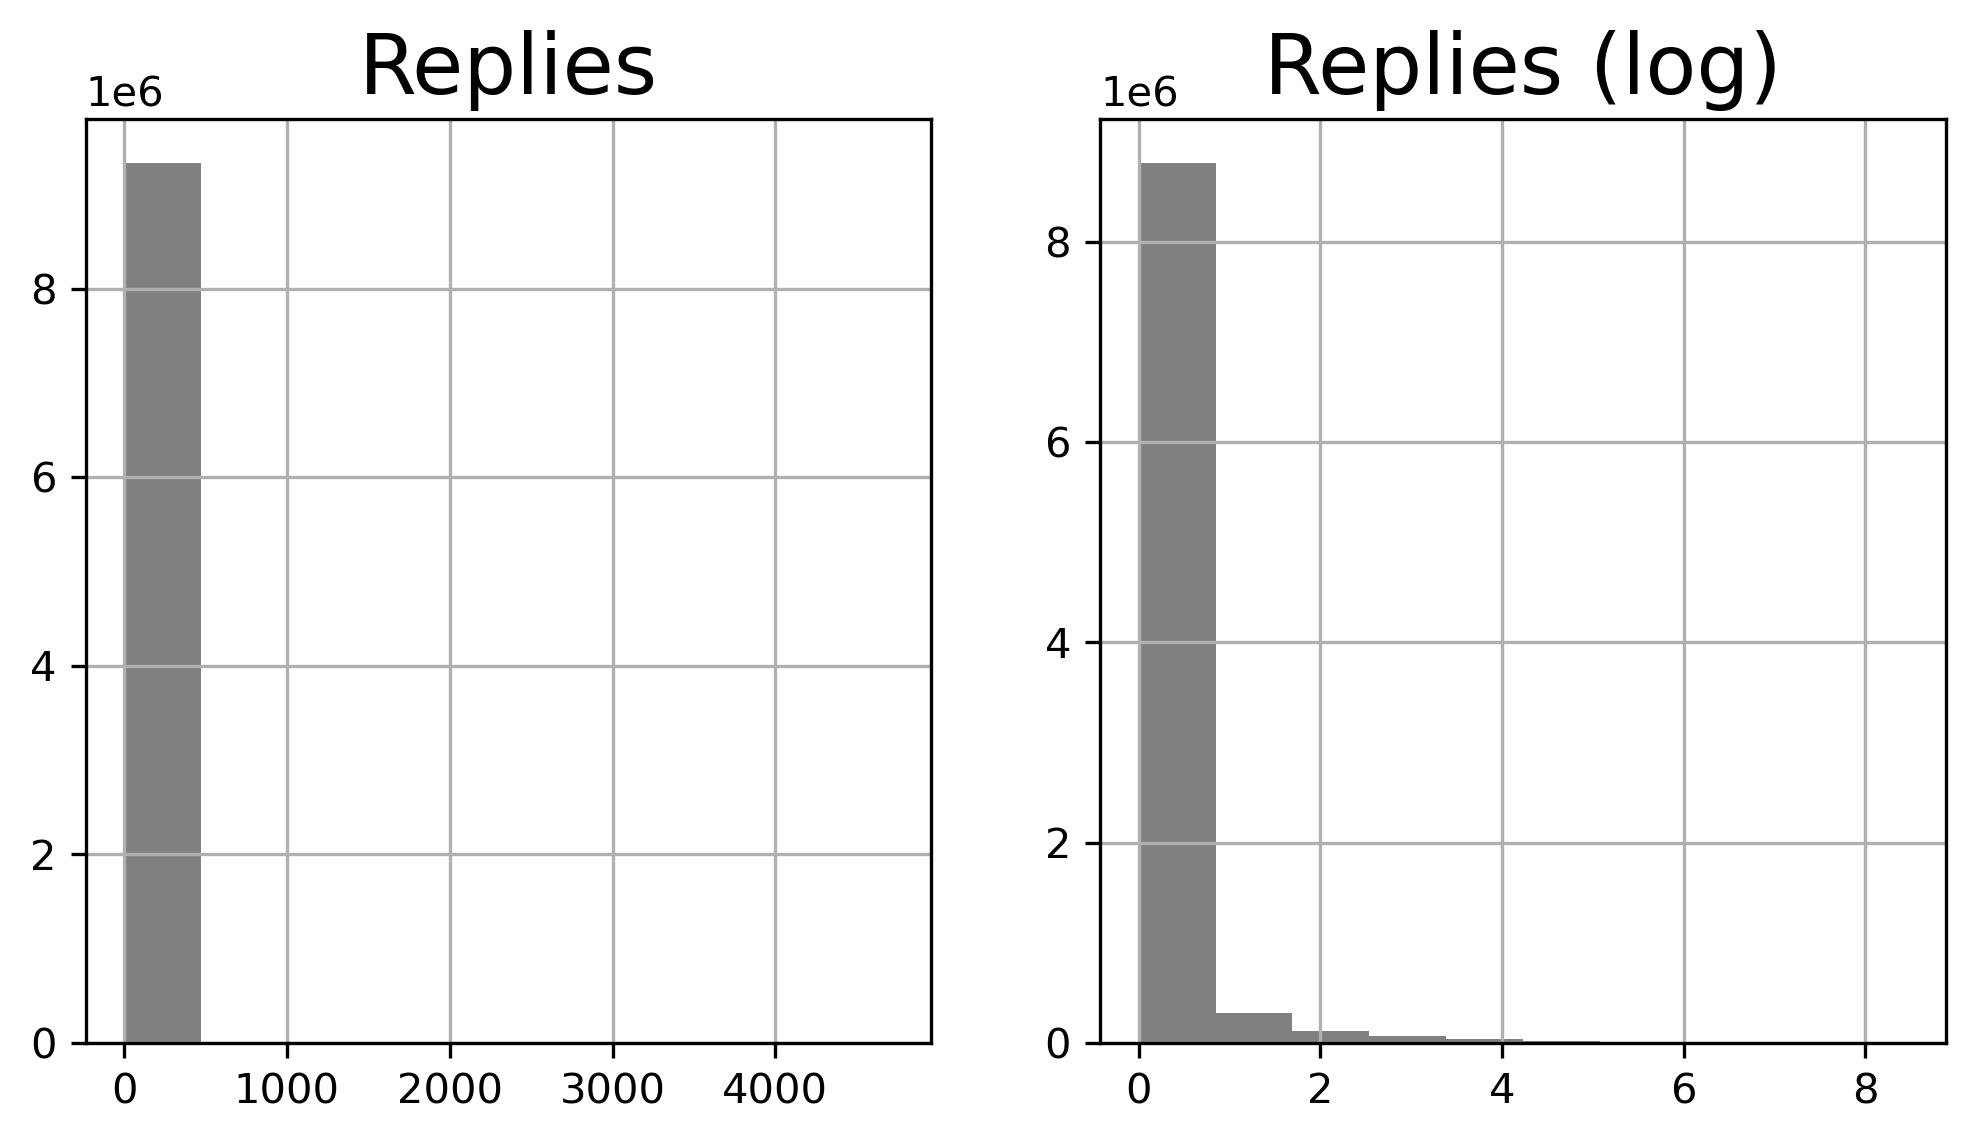
\includegraphics[width=3.125in,height=\textheight]{images/reply_distributions.png}

Zeileis et al., \href{http://www.jstatsoft.org/v27/i08/}{2008}



\end{document}
